%!TEX root = ../document.tex
\chapter{Lösungsansatz} \label{chp:Loesungsansatz}
	
	\section{Überblick} 

		Die Bestimmung der geografischen Position, von der ein Tweet abgesetzt wurde, soll durch die Auswertung des Nutzer-Standortfeldes erfolgen. 
		Der Lösungsansatz besteht aus den folgenden zwei Teilen:

		\begin{enumerate}
			\item Training: Lernverfahren zur Erzeugung einer Wissensdatenbank 
			\item Geolokalisierung: Auflösen des Nutzer-Standortes durch die Verarbeitung der Informationen aus der Wissensdatenbank
		\end{enumerate}

		Beim Training soll aus einer Menge an Trainingsdaten eine Wissensdatenbank (im folgenden Georeferenz-Basis genannt) generiert werden.
		Es soll dabei die quantitative Verteilung der Werte des Nutzer-Standortes erfasst werden.
		Jeder Trainingsdatensatz repräsentiert einen Tweet, der den Nutzer-Standort, die Nutzer-Zeitzone und geografische Koordinaten beinhaltet.
		Die Nutzer-Zeitzone wird verwendet um Doppel- und Mehrdeutigkeiten bezüglich der Werte im Nutzer-Standort auflösen zu können. 
		Aus diesen Trainingsdatensätzen kann durch die Untersuchung der Nutzer-Standorte und der zugehörigen geografischen Koordinaten bestimmt werden wie oft ein Wert an einer bestimmten geografischen Position vorkommt.

		Bei der Geolokalisierung soll ein gegebener Nutzer-Standort auf eine Georeferenz aufgelöst werden. 
		Dies geschieht durch eine Abfrage der Werte im Nutzer-Standort an die Georeferenz-Basis.
		Es werden daraufhin Ergebnisdatensätze zurückgeliefert, welche die geografische Verteilung des entsprechenden Wertes widerspiegeln.
		Durch eine Analyse der Verteilungen soll entschieden werden welcher der zurückgelieferten Ergebnisdatensätze am wahrscheinlichsten die korrekte geografische Position, von welcher der Tweet abgesetzt wurde, liefert.
		Die Güte und der Trefferquote der Ergebnisse kann dabei mit Hilfe von Schwellwerten justiert werden.
		Des weiteren kann die Hierarchieebene angegeben werden welcher das Ergebnis zuzuordnen ist.

		In Abbildung \ref{img:einteilungLoesungsansatz} sind die beiden Teile des Verfahrens und deren genereller Ablauf dargestellt.
		In den folgenden Abschnitten wird auf die einzelnen Teile und deren detaillierten Ablauf eingegangen. 
		
		Um die einzelnen Schritte für das Training und die Geolokalisierung spezifizieren zu können soll zunächst der Nutzer-Standort eingehend untersucht werden.
		Dazu wird in einem ersten Abschnitt die Datenbasis vorgestellt.
		Danach wird eine quantitative Bewertung des Nutzer-Standortes vorgenommen bevor die Herausforderungen erläutert werden die bei der Verwendung des Nutzer-Stadortes als geografsicher Indikator bestehen.
		Es wird in Abschnitt \ref{sec:VefrahrenZumEinlernen} basierend auf den Ergebnissen ein Verfahrensablauf zum Training entwickelt. 
		In Abschnitt \ref{sec:AufloesenDesNutzerStandortes} wird die Geolokalisierung, welche die eingelernte Georeferenz-Basis aus dem Training verwendet.
		Dabei werden Schwellwerte zur Justierung der Güte und Trefferquote eingeführt.
		Im letzten Abschnitt \ref{sec:ausnutzenDerGeografischenHierarchie} wird vorgestellt wie die geografische Hierarchie einbezogen wird.

		\textit{Stand der Technik} 

	\section{Verwendete Datenbasis}

		In diesem Abschnitt wird die Datenerhebung und die daraus resultierenden Datensätze betrachtet.
		Zunächst wird aufgezeigt wie die Daten erhoben wurden, und daraus die Trainingsdatensätze sowie Testdatensätze generiert wurden.
		Zudem werden 1000 Tweets per Hand auf die grundsätzliche Eignung als geografischer Indikator untersucht.
		Es werden dabei quantitative Daten zu geografischem Bezug des Nutzer-Standortes erhoben.
		In einem weiteren Abschnitt werden die Herausforderungen betrachtet die bei der Verwendung des Nutzer-Standortes als geografischer Indikator entstehen. 
		Diese sind weitestgehend der freien unkontrollierten Eingabe des Nutzers geschuldet.

		\subsection{Datenerhebung} 

			Die Trainingsdatensätze und die Testdatensätze, die später zur Evaluierung verwendet werden, wurden als zufällige Samples aus einem größeren Datensatz erzeugt.
			Der Datensatz wurde mit Hilfe der Twitter Streaming API erzeugt.
			Die Twitter Streaming API bietet die Möglichkeit ausschließlich Tweets, welche einen Längen- und Breitengrad als Positionsangabe besitzen, abzufragen.
			Bei der näheren Betrachtung hat sich jedoch herausgestellt, dass viele der Tweets für den Längen- und den Breitengrad die Werte (0,0) enthalten. 
			Dies beschreibt eine Position im Golf von Guinea vor der Küste West-Afrikas. 
			Es ist davon auszugehen, dass die 65428 Tweets welche diese Angabe als geografische Koordinaten besitzen nicht von dort versendet wurden.
			Diese wurden aus dem Datensatz entfernt.
			Des weiteren wurden Tweets ohne Werte im Nutzer-Standort entfernt, da diese weder für das Training noch für die Evaluierung genutzt werden können.
			Daraus resultiert eine Basis an Datensätzen mit 383222 Tweets aus dem die Trainingsdatensätze und die Testdatensätze erzeugt werden.  
			Der Testdatensatz besteht aus 20000 zufällig gesampelten Tweets aus diesen Basisdatensätzen. 
			Die restlichen 383222 Tweets werden als Lerndatensätze verwendet. 

				\begin{table}[h]
				\centering
				\caption{Basisdatensätze}
				\label{my-label}
				\begin{tabular}{|l||l|}
				\hline
				Zeitraum & \begin{tabular}[c]{@{}l@{}}23.01.2014 12:00 Uhr\\ bis  04.02.2014 21:00 Uhr\end{tabular} \\ \hline
				Gesamtanzahl Tweets							 & 623645  \\ \hline
				Tweets ohne valide geografische Koordinaten  &	65428    \\ \hline
				Tweets ohne Nutzer-Standort 				 & 169320  \\ \hline
				\begin{tabular}[c]{@{}l@{}}Ohne Nutzer-Stadort und\\ geografische Koordinaten nicht valide\end{tabular} & 65428 \\ \hline
				Basis zur Erzeugung Lerndatensätze und Testdatensätze & 403222 \\ \hline
				Lerndatensätze & 383222 \\ \hline
				Testdatensätze & 20000  \\ \hline
				\end{tabular}
				\end{table}

	\section{Bewertung des Nutzer-Standortes}

		In diesem Abschnitt soll untersucht werden in wie vielen Fällen dem Nutzer-Standort geografischer Bezug nachgewiesen werden kann.
		Dabei werden zum Nutzer-Standort quantitative Daten erhoben um die Eignung des Nutzer-Standortes zur Geolokalisierung zu überprüfen.

		\subsection{Methodik zur Untersuchung des Nutzer-Standortes}

			Aus den Basisdatensätzen wurden zufällig 1000 Tweets gewählt. 
			Es wurde eine Oberfläche zur Untersuchung der Nutzer-Standorte dieser 1000 Tweets erstellt.
			Die Oberfläche bietet die Möglichkeit in Google-Maps oder auf dem Ortsverzeichnis von geonames.org nach Toponymen zu suchen.
			Wurde ein Toponym per Suche gefunden wurde dieses dem Datensatz zugeordnet.

			In Abbildung \ref{img:oberflaecheQuantitative} ist die Oberfläche zur Untersuchung von Nutzer-Standorten dargestellt. 
			Der aktuelle Nutzer-Standort wird in der Leiste oben angezeigt, hier Istanbul. 
			Auf der linken Karte wird das Ergebnis von Google-Maps angezeigt.
			Rechts kann im geonames.org Ortsverzeichnis gesucht werden. 
			Die gefundenen Datensätze werden in der Liste rechts angezeigt.  
			In der rechten Karte kann man sich mit einem Klick auf "'in Karte anzeigen"'' den jeweiligen geonames.org Datensatz aus der Liste anzeigen lassen.

			\begin{figure}[!ht]
					\begin{center}
						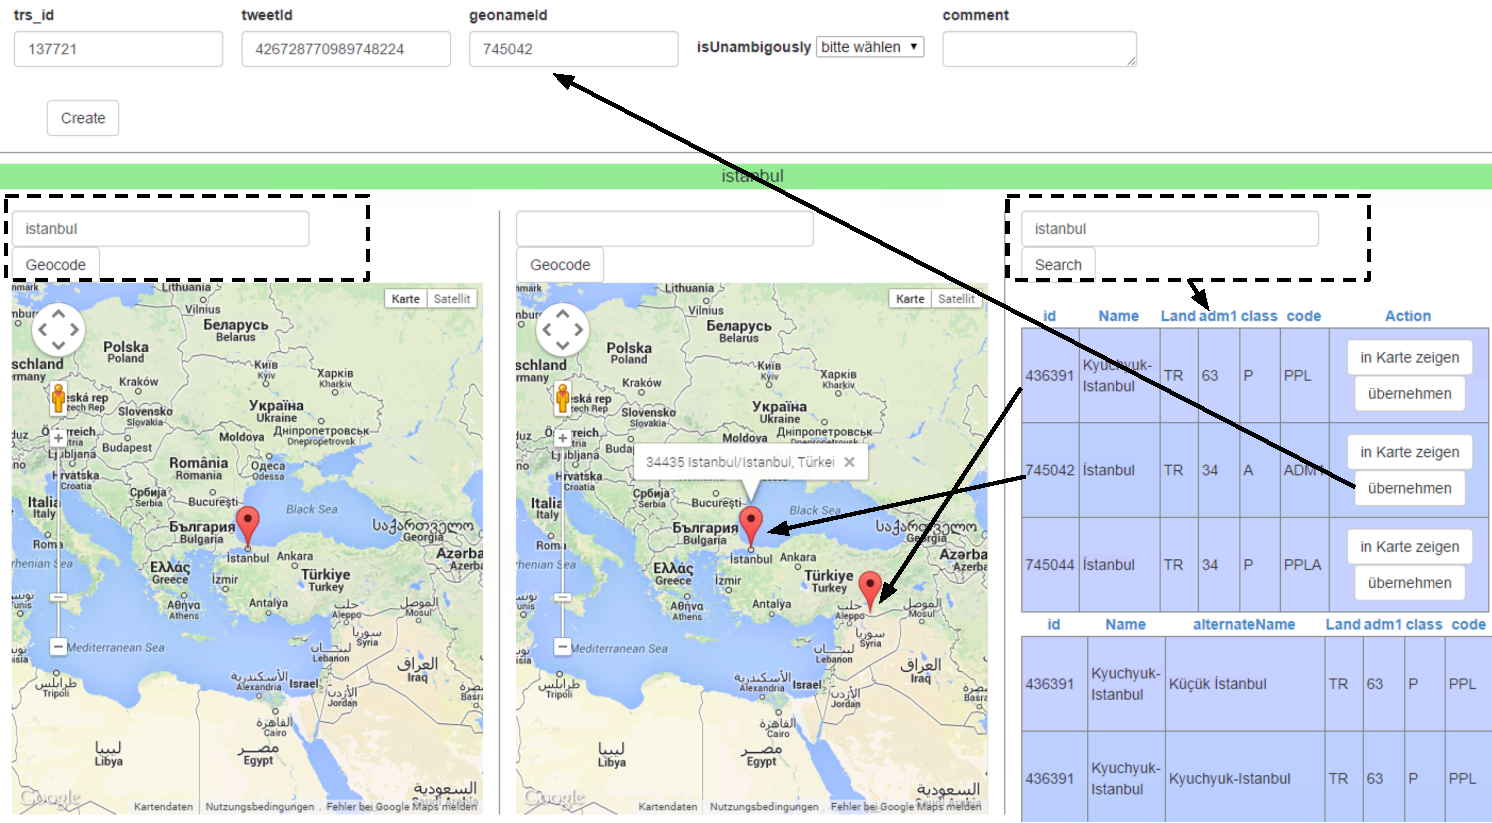
\includegraphics[scale=0.5]{_oberflaecheQuantitative.pdf}
						\caption{Oberfläche zur Untersuchung des Nutzer-Standortes}
						\label{img:oberflaecheQuantitative}
					\end{center}  
			\end{figure}	

			Die mit dieser Oberfläche erhobenen Daten wurden untersucht. 
			Die Ergebnisse werden in den folgenden Abschnitten vorgestellt.
			Es wurde über Google-Maos und geonames.org versucht den Nutzer-Standort zuzuordnen. 
			Auch wenn die Sprache oder das verwendete Alphabet nicht bekannt waren wurde eine Georeferenz zugeordnet sofern die Suche auf den Ortsverzeichnissen einen Treffer ergab. 


	
			\todo{chap: Lösungsanatz sec: Untersuchung der Werte ---> die nächsten vier Kapitel: Hecht in Grundlagen, meine Untersuchungen hier lassen unter Methodik} 

		\subsection{Geografischer Bezug des Nutzer-Standortes} 
			
			In den eigenen Untersuchungen konnten 76\% der Nutzer-Standorte ein geografischer Bezug nachgewiesen werden. 
			Wurde geografischer Bezug nachgewiesen, so musste der Wert des Nutzer-Standortes im Ortsverzeichnis von geonames.org vorkommen. 
			Daraus kann gefolgert werden, dass in 76\% der Fälle ein Toponym im Nutzer-Standort vorhanden ist.
			
			In den restlichen 24\% der Fälle konnte kein geografischer Bezug mit Hilfe der Ortsverzeichnisse nachgewiesen werden. 
			Dies bedeutet nicht, dass grundsätzlich kein geografischer Bezug vorhanden ist. 
			Es konnte lediglich anhand der genutzten Quellen kein geografischer Bezug hergeleitet werden.
			Beispielsweise wurde "'Swag City"', ein Beiname für die Stadt "'Ann Arbor"' denn der Spitzname für die Stadt war in den Datenbanken nicht hinterlegt. 
			Dies zeigt, dass Werte denen über ein Ortsverzeichnis keine Georeferenz zugewiesen werden konnte, durchaus geografischen Bezug haben können.
			Das verwerfen solcher Werte durch unzureichendes Wissen über Toponyme kann zum Verlust wertvoller Informationen über den tatsächlichen Standort führen.

			Hecht et al. konnten in \cite{Hecht2011} den Datenwerten in den Nutzer-Standorten in 80\% der Fälle einen geografischen Bezug feststellen.
			In den restlichen 20\% der Fälle konnte im Nutzer-Standort kein geografischer Bezug festgestellt werden. 
			Diese Ergebnisse decken sich mit den eigenen Untersuchungen. 
			Es ist allerdings zu beachten, dass Hecht et al. ausschließlich Tweets aus den USA verwendet haben und die Nutzer-Standorte nur in englischer Sprache verfasst waren. 
					
	\section{Herausforderungen bei der Verwendung des Nutzer-Standortes als geografischen Indikator} \label{sec:HerausforderungenBeiDerVerwendungDesNutzerStadortes}  

		Neben den in Kapitel \ref{sec:zuordnungToponymeGeogObj} erwähnten Problemen bei der Zuordnung von Toponymen zu geografischen Objekten sind noch weitere Probleme zu erwarten.
		Diese sind hauptsächlich bedingt durch die freie Eingabe des Nutzer-Standortes.
		Es wurden dabei folgende Klassen identifiziert in die die Werte eingeteilt werden können:

		\begin{enumerate}	
		 	\item Partieller geografischer Bezug des Wertes
		 	\item Widersprüchliche Werte 
		 	\item Geografische Hierarchien
		 	\item Domänenspezifische Toponyme (Neologismen)
		 	\item Toponyme unterschiedlicher Hierarchieebenen
		 	\item Keiner oder mittelbarer geografischer Bezug
		\end{enumerate}	 

		\subsection{Partieller geografischer Bezug des Datenwertes im Nutzer-Standort} \label{sub:partiellerGeografischerBezug} 

			Hierbei haben nur Teile des Wertes im Nutzer-Standort geografischen Bezug. 
			Im Nutzer-Standort werden oft weitere Informationen angegeben die keinen geografischen Bezug haben. 
			Im folgenden einige Beispiele.

			\begin{table}[h]
				\centering
				\caption{Beipiele für Nutzer-Standorte mit partiellem geografischen bezug}
				\label{my-label}
				\begin{tabular}{|l|l|l|}
				\hline
				\multicolumn{1}{|c|}{Wert} & \multicolumn{1}{c|}{geografischer Bezug} & \multicolumn{1}{c|}{kein geografischer Bezug} \\ \hline
				East side of that London & East side London & of that \\ \hline
				11th Dimension California & California & 11th Dimension \\ \hline
				New Orleans Home of the goons & New Orleans & Home of the goons \\ \hline
				Between here and there Miami & Miami & Between here and there \\ \hline
				\end{tabular}
			\end{table}
			
			Es können also auch nur Teile des Nutzer-Standorts für eine Geolokalisierung von Nutzen sein.
			Diese Informationen müssen extrahiert werden um einen Nutzen aus ihnen ziehen zu können. 

		\subsection{Widersprüchliche Toponyme im Nutzer-Standort} \label{sub:wiederspruechlicheBezuege} 

			Es existieren auch Datenwerte in denen mehrere widersprüchliche Angaben gemacht werden.
			Dies bedeutet es werden zwei oder mehr Datenwerte mit geografischem Bezug angegeben, die auf unterschiedliche geografische Objekte verweisen.
			Auch hier sollen einige Beispiele genannt werden:

			\begin{table}[h]
			\centering
			\caption{Beispiele für widersprüchliche Toponyme}
			\label{my-label}
			\begin{tabular}{|l|l|l|l|}
			\hline
			\multicolumn{1}{|c|}{Wert}      & \multicolumn{1}{c|}{Toponym 1} & \multicolumn{1}{c|}{Toponym 2} & \multicolumn{1}{c|}{Entfernung in km} \\ \hline
			Bolton\textbackslash/Leigh      & Bolton                         & Leigh                          & 14 									\\ \hline
			Liverpool\textbackslash/London  & Liverpool                      & London                         & 350 								\\ \hline
			Balikesir \textbackslash/ Izmir & Balikesir                      & Izmir                          & 180 								\\ \hline
			\end{tabular}
			\end{table}					
				
			In diesen Beispielen sind jeweils zwei Städte angegeben.

			Es kann nun spekuliert werden wieso der Nutzer zwei Städte angibt.
			Ist er in einer der Städte aufgewachsen und lebt momentan in der anderen?
			Pendelt er zwischen den Städten um zu Arbeiten?

			Es kann hier nicht eindeutig entschieden werden in welcher Stadt sich der Nutzer aufhält.

		\subsection{Geografische Hierarchien im Nutzer-Standort} \label{sub:geografischeHierarchienImNutzerStandort} 

			Es ist auch möglich, dass im Nutzer-Standort teile einer geografischen Hierarchie angegeben sind.
			Beispielsweise die Angabe einer Stadt in Kombination mit einem Land.
			
			In den USA wird beispielsweise oft die Stadt und der zugehörige Bundesstaat angegeben.
			In Brasilien hingegen wird oft ein Bundesstaat und das Land angegeben.
			Hier einige Beispiele:

			\begin{table}[h]
			\centering
			\caption{Beispiele für Nutzer-Standorte mit geografischen Hierarchieebenen}
			\label{my-label}
			\begin{tabular}{|l|c|c|c|c|}
			\hline
			\multicolumn{1}{|c|}{Wert} & Stadt       & \multicolumn{1}{l|}{Adm2} & Adm1 & \multicolumn{1}{l|}{Land} \\ \hline
			Orange County, USA 		   & - 			 & Orange County										 & - 							   & USA    					\\ \hline
			Las Vegas, USA 		       & Las Vegas   & - 												     &								   & USA 					    \\ \hline
			Mato Grosso, Brazil        & -           & -                                                     & Mato Rrosso                     & Brazil                    \\ \hline
			West Sussex, England       & -           & -                                                     & West Sussex                     & England                   \\ \hline
			\end{tabular}
			\end{table}
 
			Durch die Kombination mehrerer Toponyme unterschiedlicher geografischer Hierarchieebenen wird die geografische Position näher beschrieben.
			Umso genauer eine geografische Position mit Toponymen beschrieben wird umso geringer ist die Gefahr von Doppel- und Mehrdeutigkeiten.  
			Diese Information sollte bei einer Untersuchung erhalten bleiben.
			
		\subsection{Domänenspezifische Toponyme im Nutzer-Standort (Neologismen)} \label{sub:domaenenspezBezug} 

			In sozialen Netzwerken können sich eigene Begriffe und Formulierungen etablieren. 
			Diese sind im allgemeinen nicht bekannt.


			Im Twitter-Umfeld haben sich in den letzten Jahren einige spezielle Begriffe und Formulierungen zur Verwendung in Tweet-Texten etabliert. 
			Das im Twitter-Umfeld auch spezielle Toponyme im Nutzer-Standort verwendet werden, kann nicht gänzlich ausgeschlossen werden. 

			Ein Beispiel hierfür ist "'Bieberville"', welches in den untersuchten Daten von Hecht et al. öfter vorkommt.
			"'Bieberville"' wird abgeleitet von dem Pop-Star Justin Bieber.	
			Da der Pop-Star in Twitter sehr aktiv ist und deshalb viele seiner Fans auch in Twitter aktiv sind hat sich dieser Name etabliert.
			Unter diesem Gesichtspunkt hätte "'Bieberville"' keinen geografischen Bezug.
			Sucht man im Internet nach "'Bieberville"' stößt man auf einen Imbiss in Groß-Bieberau.
			"'Bieberville"' kann also durchaus einen geografischen Bezug haben, wenngleich es im Twitter-Umfeld nicht als solcher benutzt wird. 
			Ist in einem Ortsverzeichnis beispielsweise "'Bierberville"' als Bezeichnung für den Imbiss in Groß-Bieberau hinterlegt, würde dieser als Georeferenz zugeordnet werden, was im Umfeld von Twitter in einem Großteil der Fälle falsch wäre.

			Das Wissen über die Verwendung domänenspezifischer Toponyme kann nur aus der Domäne selbst generiert.
		
		\subsection{Kein geografischer oder mittelbar geografischer Bezug} \label{sub:keinGeogOdMittelBarereBezug}

			Im Nutzer-Standortfeld können auch Werte auftauchen die keinen geografischen Bezug aufweisen.
			Beispiele hierfür sind:

			\begin{table}[h]
			\centering
			\caption{My caption}
			\label{my-label}
			\begin{tabular}{|l|}
			% hline
			Werte                      	\\ \hline
			In the middle of nowhere   	\\ \hline
			95                         	\\ \hline
			Highsociety                	\\ \hline
			cold	                 	\\ \hline
			rabbit     					\\ \hline
			\end{tabular}
			\end{table}

			Diese Werte haben auf den ersten Blick keinen geografischen Bezug.
			Es ist jedoch nicht auszuschließen, dass einige dieser Begriffe in bestimmten Regionen gehäuft auftreten.
			Damit hätten diese Begriffe geografischen Bezug.
			Dies kann bedingt durch die Landessprache oder Dialekte der Fall sein.

	\section{Verfahren zum Einlernen der Georeferenz-Basis} \label{sec:VefrahrenZumEinlernen} 	
			
			In Abbildung \ref{img:einlernenAblauf} ist der Gesamtablauf des Einlernens dargestellt. 
			Die Werte im Nutzer-Standortfeld werden zuerst einer Vorverarbeitung unterzogen. 
			Durch die Vorverarbeitung werden die Datenwerte im Nutzer-Standort vorbereitet um weitere Informationen zu extrahieren.
			Es wird danach eine Zerlegung der Werte im Nutzer-Standortfeld vorgenommen.
			Die Zerlegung extrahiert dabei zusätzliche Informationen aus dem Nutzer-Standort.
			DDie Nutzer-Zeitzone wird hinzugezogen um bei der Geolokalisierung etwaige Doppel- und Mehrdeutigkeiten von Toponymen erkennen zu können.
			Das Ergebnis dieser Schritte ist eine Menge an Referenzwerten.

			Parallel dazu werden die geografischen Koordinaten des Tweets auf eine diskrete geografische Position aufgelöst.
			Dies erfolgt durch die Zuordnung der geografischen Koordinaten zu der nächstgelegenen Stadt.

			Die Kombinationen aus Referenzwerten und diskreten geografischen Positionen werden in der Georeferenz-Basis gespeichert.
			Es wird dabei die quantitative Verteilung der Referenzwerte über den Globus erfasst.
			
			 \begin{figure}[!ht]
				\begin{center}
					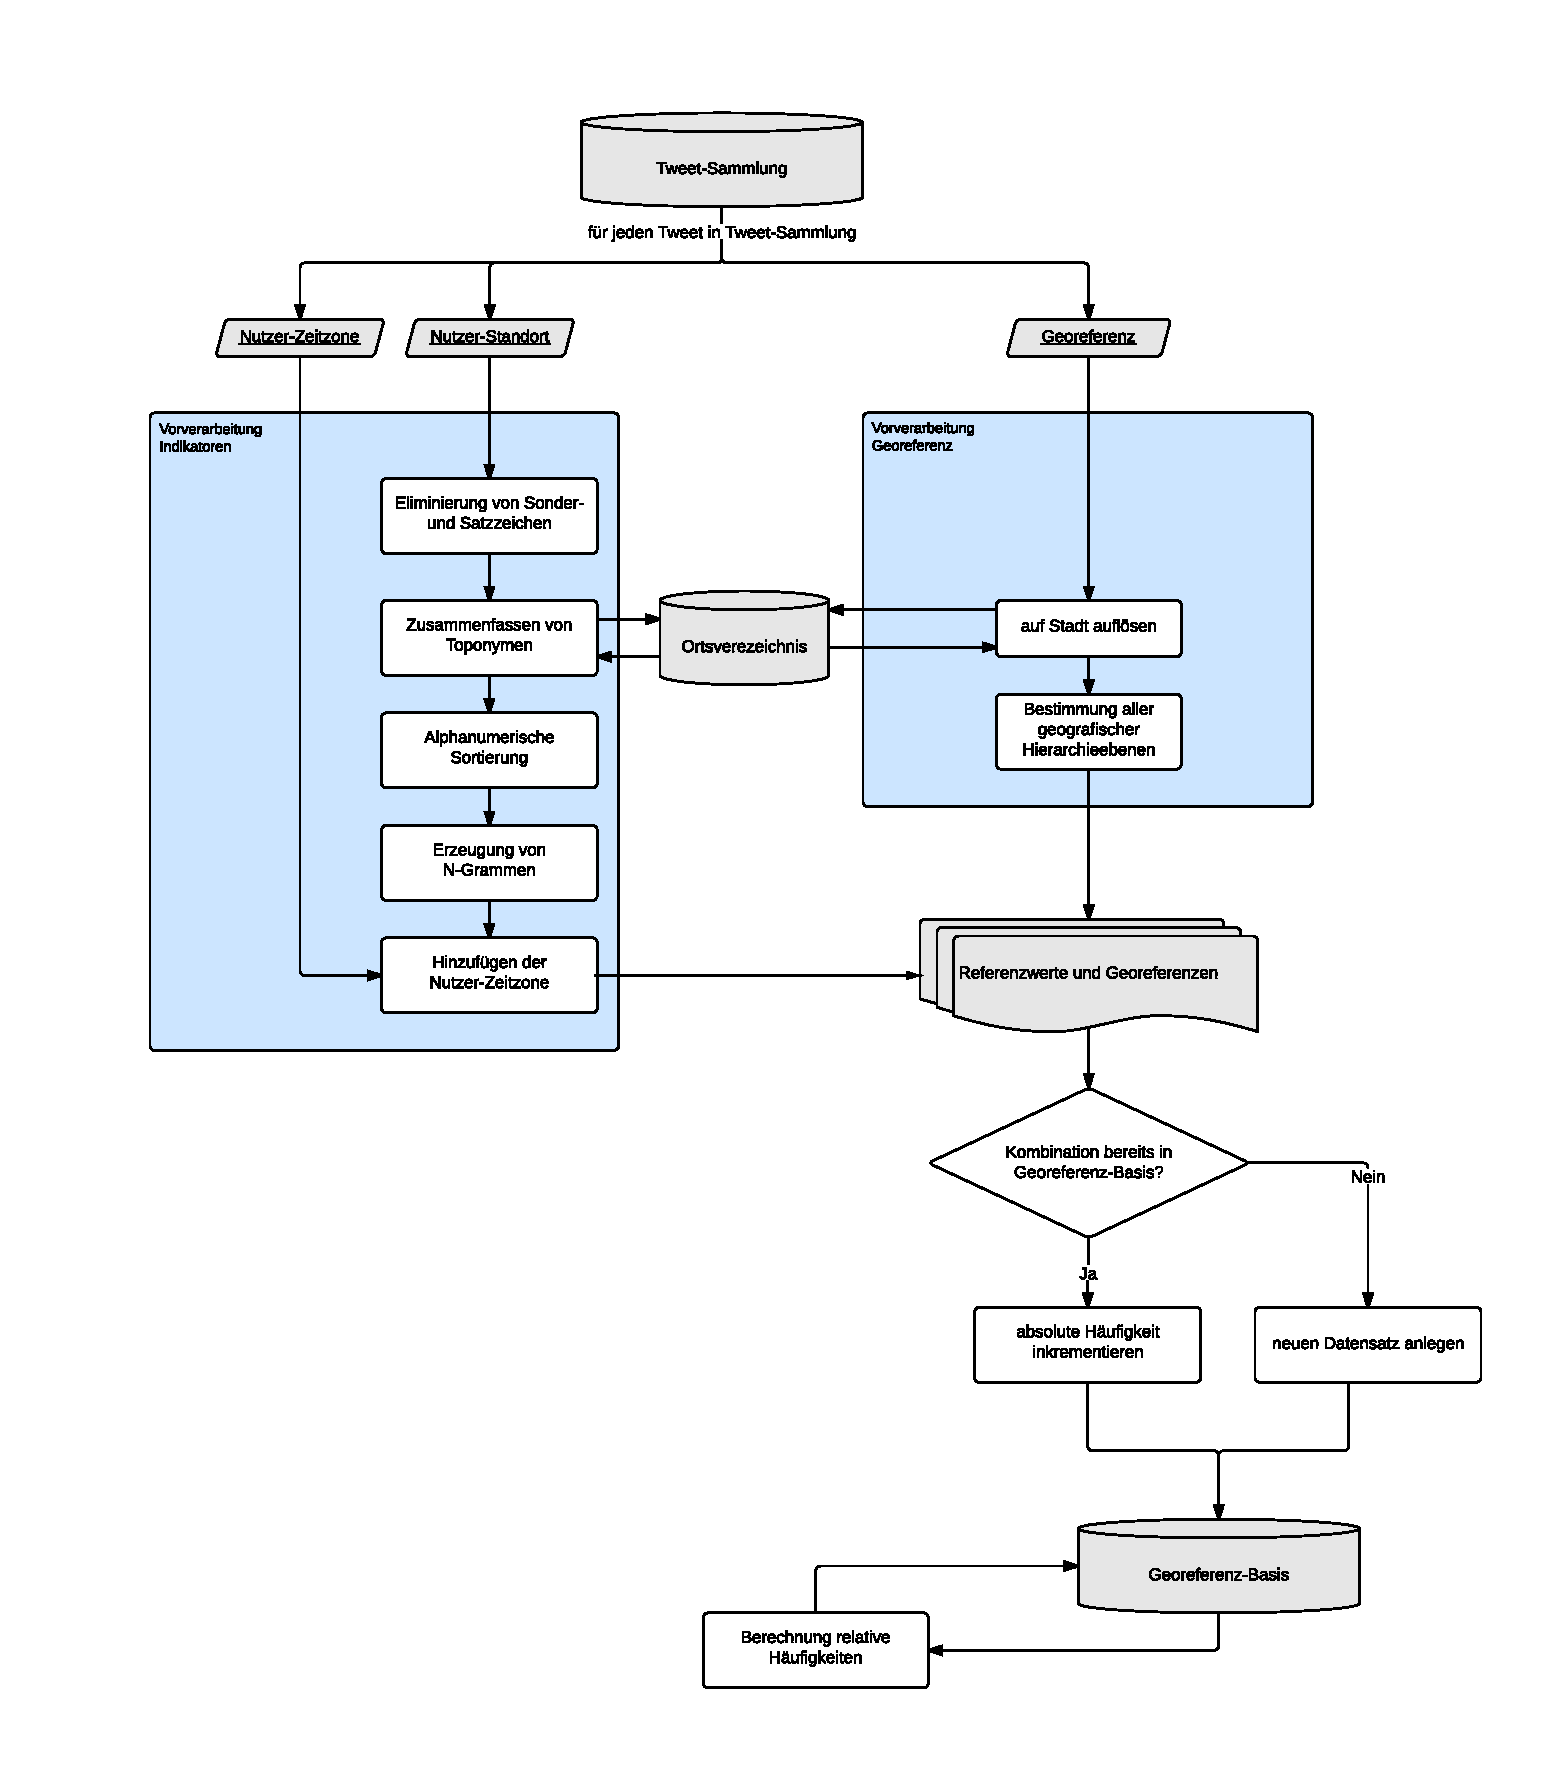
\includegraphics[scale=0.6]{einlernenAblauf.pdf}
					\caption{Ablaufplan einlernen}
					\label{img:einlernenAblauf}
				\end{center}
			\end{figure}

			Die Datenstruktur der Georeferenz-Basis beinhaltet die Referenzwerte, die zugeordnete Stadt, und die übergeordneten Hierarchieebenen. 
			Zusätzlich wird das vorkommen eines Referenzwertes in einer Stadt als absolute Häufigkeit gespeichert. 

			Durch dieses Verfahren lässt sich eine Datenbasis erzeugen die auch domänenspezifische Eigenheiten, in Bezug auf die Verwendung spezieller Begriffe oder Formulierungen, berücksichtigt.
			Des weiteren werden Toponyme, die in Ortsverzeichnissen unter Umständen nicht hinterlegt sind, berücksichtigt.
			Auch geografische Indikatoren mit mittelbarem geografischen Bezug, zum Beispiel die Verwendung spezieller Begriffe in einer geografischen Region, können einbezogen werden.

			In Tabelle \ref{tab:strukturMitHierarchie1} ist die Struktur der Georeferenz-Basis dargestellt.

			\begin{table}[htpb]
				\caption{Struktur der Georeferenz-Basis mit geografischer Hierarchie} 
				\centering
				\tiny
				\begin{tabular}{|c|c|c|c|c|c|}
					\hline
					Referenzwert & Stadt & Adm2 & Adm1 & Land & abs. Häufigkeit \\
					\hline\hline
					 "'LA"' & Los Angeles & LA County & CA & USA & 30 \\
					\hline
					 "'San Francisco"'   & San Francisco & SF County & CA & USA & 3 \\
					\hline
					 "'Los Angeles"'   & Los Angeles & LA County & CA & USA & 70 \\
					\hline
					 "'Stuttgart"'   & Stuttgart & Regierungsbezirk Stuttgart & BaWü & BRD & 80 \\
					\hline
					 "'London City"'   & London & City London & Greater London & GB & 90\\
					\hline
				\end{tabular}
				\label{tab:strukturMitHierarchie1} 
			\end{table}  		
		
		\subsection{Schritte zur Vorverarbeitung der Werte des Nutzer-Standortfeldes}

			Die Werte des Nutzer-Standortfeldes wird einer Vorverarbeitung unterzogen.
			In Abbildung \ref{img:vorverarbeitung} sind die einzelnen Schritte dargestellt.
			Die Vorverarbeitung ist notwendig um die Werte auf die Extrahierung weiterer Daten vorzubereiten.
			Die einzelnen Worte im Nutzer-Stadort werden als Token bezeichnet. 
			
			Es sollen zunächst Sonder- und Satzzeichen entfernt werden, diesen kann in der Regel kein geografischer Bezug nachgewiesen werden.
			In einem weiteren Schritt werden mit Hilfe eines Ortsverzeichnisses zwei oder mehr Token, die gemeinsam ein Toponym darstellen, zusammengefasst.
			Danach wird eine alphanumerische Sortierung der Token durchgeführt.

			In Tabelle \ref{tab:VorverarbeitungBsp1} sind einige Werte von Nutzer-Standortfeldern aufgeführt.
			Diese sollen in den folgenden Abschnitten als durchgängiges Beispiel verwendet werden.

				\begin{table}[h]
					\centering
					\caption{Beispielwerte}
					\label{tab:VorverarbeitungBsp1}
					\begin{tabular}{|l|l|}
					\hline 
					\multicolumn{2}{|c|}{\textbf{Werte Nutzer-Standortfeld}} \\ \hline \hline
					1&Mato Grosso \& Rio de Janeiro                      			\\ \hline
					2&\_***\_                                         			\\ \hline
					3&USA\textbackslash /Los Angeles                  			\\ \hline
					4&Los Angeles, USA                                			\\ \hline
					5&$\dagger$\textasciitilde York \textasciitilde$\dagger$      \\ \hline
					6&Nottingham\textbackslash /London                			\\ \hline
					7&York                                            			\\ \hline
					8&11th Dimension | California 					\\ \hline	
					\end{tabular}
				\end{table} 
			 
			\subsubsection{Eliminierung von Sonder- und Satzzeichen} 

				Es werden oft Sonder- und Satzzeichen im Nutzer-Standort verwendet. 
				Beispielsweise als Trenner zwischen Toponymen unterschiedlicher geografischer Hierarchieebenen.
				Beispiele hierfür sind die Zeilen 1,3 und 6 in Tabelle \ref{tab:VorverarbeitungSonder}. 
				Die Trennzeichen werden nicht einheitlich verwendet.
				Weder die Rangfolge der Hierarchieebene noch das verwendete Satzzeichen sind einheitlich.  
				Es ist also nicht klar welcher Zusammenhang zwischen den Datenwerten, die durch ein Sonder- oder Satzzeichen getrennt werden, besteht. 

				Auch werden Sonder- und Satzzeichen ausschließlich oder als Dekoration verwendet Beispiele hierfür sind die Zeilen 2 und 5 in Tabelle \ref{tab:VorverarbeitungSonder}.
				In den oben genannten Fällen bringen Sonder- und Satzzeichen keine zusätzlichen Informationen.
				Es sollen deshalb in einem ersten Vorverarbeitungsschritt alle Sonder- und Satzzeichen entfernt werden. 

				Liste nach dem entfernen von Sonder- und Satzzeichen:

				\begin{table}[h]
				\centering
				\caption{Eliminierung von Sonder- und Satzzeichen}
				\label{tab:VorverarbeitungSonder}
				\begin{tabular}{|l|l|l|}
				\hline \hline
				  & \multicolumn{1}{c|}{\textbf{Vorher}} & \multicolumn{1}{c|}{\textbf{Nachher}} \\ \hline
				1 & Mato Grosso \& Rio de Janeiro        & Mato Grosso Rio de Janeiro            \\ \hline
				2 & \_***\_                              &                                       \\ \hline
				3 & USA\textbackslash /Los Angeles       & USA Los Angeles                       \\ \hline
				4 & Los Angeles, USA                     & Los Angeles USA                       \\ \hline
				5 & $\dagger$\textasciitilde York \textasciitilde$\dagger$                             & York                                  \\ \hline
				6 & Nottingham\textbackslash /London     & Nottingham London                     \\ \hline
				\end{tabular}
				\end{table}

				Der Wert 6 existiert nun nicht mehr, der Wert ist leer und wird somit nicht weiter betrachtet.

			\subsubsection{Zusammenfassen von Toponymen mit Hilfe von a priori Wissen aus einem Ortsverzeichnis}

				Oft bestehen Toponyme aus zwei oder mehr Token.
				Diese sollen mit Hilfe eines Ortsverzeichnisses zusammengefasst werden. 
				Dies kann selbstverständlich nur für bekannte Toponyme durchgeführt werden.
				
				"'Los"' und "'Angeles"' bilden gemeinsam "'Los Angeles"' und sollen in der weiteren Verarbeitung gemeinsam betrachtet werden. 
				Dies soll zunächst mit einem + Zeichen gekennzeichnet werden.

				Daraus resultiert:

				\begin{table}[h]
				\centering
				\caption{Zusammenfassen von Toponymen}
				\label{tab:VorverarbeitungZusammen}
				\begin{tabular}{|l|l|l|}
				\hline
				  & \multicolumn{1}{c|}{\textbf{Vorher}} & \multicolumn{1}{c|}{\textbf{Nachher}} \\ \hline \hline
				1 & Mato Grosso Rio de Janeiro           & Mato+Grosso Rio+de+Janeiro            \\ \hline
				2 &                                      &                                       \\ \hline
				3 & USA Los Angeles                      & USA Los+Angeles                       \\ \hline
				4 & Nottingham London                    & Nottingham London                     \\ \hline
				5 & Los Angeles USA                      & Los+Angeles USA                       \\ \hline
				6 & York                                 & York                                  \\ \hline
				7 & 11th Dimension California            & 11th Dimension California             \\ \hline
				\end{tabular}
				\end{table}

				In diesem Schritt wird keine Geolokalisierung vorgenommen es werden lediglich Toponyme die aus zwei oder mehr Token bestehen identifiziert.
				Er dient dazu möglichst früh vorhandenes Wissen über Toponyme einzubeziehen und zusammengehörige Toponyme in den nächsten Schritten als ein Token zu behandeln.

			\subsubsection{Angleichung durch alphanumerische Sortierung}

				In diesem Schritt sollen die Token alphanumerisch sortiert werden. 
				Wenn Toponyme unterschiedlicher geografischer Hierarchieebenen angegeben sind spielt es keine Rolle mehr in welcher Reihenfolge diese angegeben werden.

				\begin{table}[h]
				\centering
				\caption{Alphanumerische Sortierung}
				\label{tab:VorverarbeitungAlpha}
				\begin{tabular}{|l|l|l|}
				\hline
				  & \multicolumn{1}{c|}{\textbf{Vorher}} & \multicolumn{1}{c|}{\textbf{Nachher}} \\ \hline
				1 & Mato+Grosso Rio+de+Janeiro           & Mato+Grosso Rio+de+Janeiro            \\ \hline
				2 &                                      &                                       \\ \hline
				3 & USA Los+Angeles                      & Los+Angeles USA                       \\ \hline
				4 & Nottingham London                    & London Nottingham                     \\ \hline
				5 & Los+Angeles USA                      & Los+Angeles USA                       \\ \hline
				6 & York                                 & York                                  \\ \hline
				7 & 11th Dimension California            & 11th California Dimension             \\ \hline
				\end{tabular}
				\end{table}

				In den Zeilen 3 und 5 in Tabelle \ref{tab:VorverarbeitungAlpha} ist nun die Reihenfolge der Toponyme angeglichen. 
				
				Dieser Schritt stellt einen Kompromiss dar.
				Es werden zwar Werte mit gleichem Inhalt und unterschiedlicher Reihenfolge angeglichen.
				Aber es werden auch potenzielle Toponyme, die aus mehreren Token bestehen, auseinandergezogen.
				Als Beispiel soll hier "'Motor City Michigan USA"' betrachtet werden.
				Wenn "'Motor City"' nicht im Ortsverzeichnis hinterlegt ist entsteht durch die alphanumerische Sortierung "'City Michigan Motor USA"'.
				Der Zusammenhang zwischen Motor und City wäre nicht mehr vorhanden und kann nicht wiedergewonnen werden.

		\subsection{Zerlegung der Werte im Nutzer-Standortfeld} 

			Als Eingabe wird in diesem Schritt das Ergebnis der Vorverarbeitung genutzt. 
			Pro Nutzer-Standortfeld existieren ein oder mehrere Token. 
			Ist nur ein Token vorhanden so wird dieser direkt weiter verarbeitet.
			Sind mehrere Token vorhanden so können diese partiellen geografischen Bezug aufweisen (siehe Abschnitt \ref{sub:partiellerGeografischerBezug}) oder eine Hierarchie darstellen (siehe Abschnitt \ref{sub:geografischeHierarchienImNutzerStandort}).
			Durch die Zerlegung sollen einzelne Token für die Weiterverarbeitung extrahiert werden.
			Im diesem Fall soll es ermöglicht werden Token mit geografischem Bezug von solchen ohne geografischen Bezug zu trennen um diese separat weiterverarbeiten zu können.
			Um allerdings die zusätzlichen Informationen, die durch die Angabe einer geografischen Hierarchie entstehen zu erhalten, sollen auch mehrere Token gemeinsam weiterverarbeitet werden können.
			Das bedeutet, der Zusammenhang mehrere Token die in einer gewissen Reihenfolge auftreten soll erhalten bleiben. 
			Um dies zu erzielen werden die Token in sogenannte N-Gramme zerlegt. 

			\subsubsection{N-Gramme}

				Eine Gruppe von Token soll derart zerlegt werden, dass sowohl einzelne Token betrachtet werden können als auch der Zusammenhang zwischen den Token, der durch ihre Reihenfolge  besteht, erhalten bleibt.
				Um dies umzusetzen soll eine Menge von Token in N-Gramme zerlegt werden.

				Die Zerlegung in N-Gramme findet unter anderem Anwendung in der Computerlinguistik und quantitativen Linguistik.
				N-Gramme bestehen aus ein oder mehreren Wörtern, die aus einem Text extrahiert werden. 
				Im vorliegenden Fall sollen die Token aus dem Nutzer-Standortfeld betrachtet werden.
				Die Extrahierung erfolgt dabei derart, dass immer zwei oder mehr aufeinanderfolgende Token zusammengefasst werden.    
				Ein Spezialfall sind Uni-Gramme, hierbei wird die Menge an Token in die einzelnen Token zerlegt.
				Bi-Gramme bestehen aus jeweils zwei aufeinanderfolgenden Token.
				Tri-Gramme bestehen aus drei aufeinanderfolgenden Token. 
				Die Anzahl der Token aus der ein N-Gramm besteht, wird auch Grad des N-Grammes genannt.

				In Tabelle \ref{tab:ngramize} wird der Ablauf zur Erzeugung von N-Grammen bis zum Grad 3 Schrittweise dargestellt.
				In Schritt 1,2 und 3 werden Uni-Gramme erzeugt. 
				Diese bestehen jeweils aus einem Token.
				In den Zeilen 4 und 5 sind die beiden Bi-Gramme dargestellt.
				In Zeile 6 schließlich wird das Tri-Gramm dargestellt. 

				\begin{table}[h]
				\centering
				\caption{Beispiel zur Erzeugung von N-Grammen}
				\label{tab:ngramize}
				\begin{tabular}{|c||l|l|l||l|}
				\hline
				 & \multicolumn{1}{c|}{0}    & \multicolumn{1}{c|}{1}         & \multicolumn{1}{c|}{2}          & Ordnung \\ \hline \hline
				0       & 11th                      & Dimension                      & California                      & -       \\ \hline
				1       & \textless 11th \textgreater &                                &                                 & 1       \\ \hline
				2       &                           & \textless Dimension\textgreater &                                 & 1       \\ \hline
				3       &                           &                                & \textless California\textgreater & 1       \\ \hline
				4       & \textless 11th\textgreater & \textless Dimension\textgreater &                                 & 2       \\ \hline
				5       &                           & \textless Dimension\textgreater & \textless California\textgreater & 2       \\ \hline
				6       & \textless 11th\textgreater & \textless Dimension\textgreater & \textless Calforinia\textgreater & 3       \\ \hline
				\end{tabular}
				\end{table}

				 
				
				In Tabelle \ref{tab:NGramme} sind alle N-Gramme zu den Beispielen aus Tabelle \ref{tab:VorverarbeitungAlpha} dargestellt.

					\begin{table}[h]
					\centering
					\caption{Zerlegung in N-Gramme}
					\label{tab:NGramme}
					\begin{tabular}{|l|l|l|}
					\hline 
					\multicolumn{1}{|c|}{\textbf{}} & \multicolumn{1}{c|}{\textbf{Vorher}}        & \multicolumn{1}{c|}{\textbf{Nachher}}                                                    \\ \hline \hline
					\multirow{3}{*}{1}              & \multirow{3}{*}{Mato+Grosso Rio+de+Janeiro} & \textless Mato+Grosso\textgreater\textless Rio+de+Janeiro\textgreater                     \\ \cline{3-3} 
					                                &                                             & \textless Mato+Grosso\textgreater                                                         \\ \cline{3-3} 
					                                &                                             & \textless Rio+de+Janeiro\textgreater                                                     \\ \hline \hline
					2                               &                                             &                                                                                          \\ \hline \hline
					\multirow{3}{*}{3}              & \multirow{3}{*}{Los+Angeles USA}            & \textless Los+Angeles\textgreater\textless USA\textgreater                                 \\ \cline{3-3} 
					                                &                                             & \textless Los+Angeles\textgreater                                                         \\ \cline{3-3} 
					                                &                                             & \textless USA\textgreater                                                                 \\ \hline \hline
					\multirow{3}{*}{4}              & \multirow{3}{*}{London Nottingham}          & \textless London\textgreater\textless Nottingham\textgreater                               \\ \cline{3-3} 
					                                &                                             & \textless London\textgreater                                                              \\ \cline{3-3} 
					                                &                                             & \textless Nottingham\textgreater                                                          \\ \hline \hline
					5                               & Los+Angeles USA                             &                                                                                          \\ \hline \hline
					6                               & York                                        & \textless York\textgreater                                                                \\ \hline \hline
					\multirow{6}{*}{7}              & \multirow{6}{*}{11th Dimension California}  & \textless 11th\textgreater\textless California\textgreater\textless Dimension\textgreater \\ \cline{3-3} 
					                                &                                             & \textless 11th\textgreater                                                                \\ \cline{3-3} 
					                                &                                             & \textless California\textgreater                                                         \\ \cline{3-3} 
					                                &                                             & \textless Dimension\textgreater                                                          \\ \cline{3-3} 
					                                &                                             & \textless 11th\textgreater\textless California\textgreater                                 \\ \cline{3-3} 
					                                &                                             & \textless California\textgreater\textless Dimension\textgreater                           \\ \hline
					\end{tabular}
					\end{table}

				Mit diesem Vorgehen können aus einer Menge Token, bei denen nur einzelne geografischen Bezug aufweisen, extrahiert werden.
				In Tabelle \ref{tab:NGramme} in Zeile 7 ist dies beispielsweise der Wert "'California"'. 
				Dieser kann im weiteren einzeln verarbeitet werden. 
				In Zeile 3 und 5 bleibt die Hierarchiebeziehung der Token im Bi-Gramm erhalten.
				Aber es können auch die einzelnen Werte mit geografischem Bezug weiter verarbeitet werden, da aus den Toponymen "'Los+Angeles"' und "'USA"' auch Uni-Gramme erzeugt werden.
				Der Vorteil der Zerlegung durch N-Gramme besteht darin, dass Token einzeln oder im Zusammenhang betrachtet werden können. 
				Somit kann aus einer Menge Token mehr Information extrahiert werden, als wenn diese gemeinsam oder ausschließlich einzeln betrachtet werden.

			\subsubsection{Weitere Verwendung der entstandenen N-Gramme} 

				Da hier maschinell keine Entscheidung getroffen werden kann welche Uni-, Bi- oder Tri-Gramme einen geografischen Bezug aufweisen, werden alle N-Gramme in die weitere Verarbeitung einbezogen. 			
				Es werden somit keine Token verworfen denen aufgrund von unzureichenden Informationen, beispielsweise durch ein unvollständiges Ortsverzeichnis, keine Georeferenz zugeordnet werden kann.
				Auch werden Werte mit mittelbarem geografischen Bezug in die weitere Verarbeitung einbezogen.
				Token mit und ohne geografischen Bezug werden weiter verarbeitet.
				Eine Entscheidung über den geografischen Bezug wird erst während der Geolokalsierung getroffen.

		\subsection{Eliminierung von Mehr- und Doppeldeutigkeiten}

				In Kapitel \ref{sec:zuordnungToponymeGeogObj} wurde auf die Probleme bei der Zuordnung von Toponymen zu geografischen Objekten eingegangen.
				Dabei wurde die Mehr- und Doppeldeutigkeit von Toponymen betrachtet.
				In den N-Grammen kann dieses Problem nach wie vor auftauchen.
				Dies ist genau dann der Fall wenn ein N-Gramm ein Toponym darstellt.

				Um diesem Problem zu begegnen soll die Nutzer-Zeitzone als weiterer geografischer Indikator hinzugezogen werden.
				Zunächst sollen die generellen Eigenschaften der Nutzer-Zeitzone erläutert werden bevor erklärt wird wie die Nutzer-Zeitzone das Problem der Mehr- und Doppeldeutigkeit von Toponymen beheben kann.

				\subsubsection{Eigenschaften der Nutzer-Zeitzone}

					Eine Zeitzone beschreibt eine eindeutige geografische Region auf dem Globus und hat somit unmittelbaren geografischen Bezug.
					Dabei entsprechen die Grenzen der Zeitzonen-Regionen nicht unbedingt den Landesgrenzen oder den Grenzen sonstiger Verwaltungseinheiten. 
					In Abbildung \ref{img:timezones} sind die Zeitzonen der Erde dargestellt.

					\begin{figure}[!ht]
						\begin{center}
							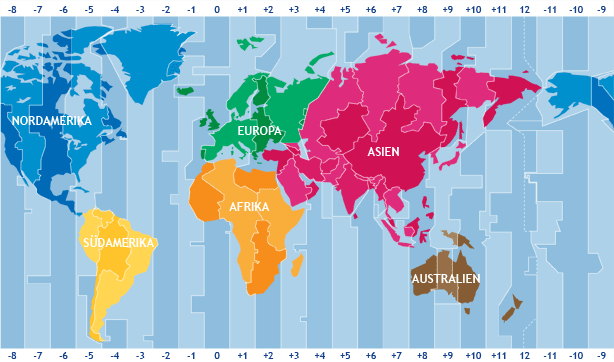
\includegraphics[scale=0.5]{zeitzonen_weltkarte.jpg}
							\caption{Zeitzonen der Erde.}
							\label{img:timezones}
						\end{center}
					\end{figure}	
					%Quelle: http://www.zeitzonen.de/images/frontend/mod\_tz\_map/zeitzonen\_weltkarte.gif

				\subsubsection{Eignung der Nutzer-Zeitzone zur Eliminierung von Mehr- und Doppeldeutigkeiten}

					In Abbildung \ref{img:usTimezones} wurden Tweets anhand ihres Längen- und Breitengrades platziert.
					Jeder Punkt in der Abbildung entspricht einem Tweet.
					Es wurden nur Tweets aus den USA ausgewählt.
					Anhand der Nutzer-Zeitzone wurde jedem Tweet eine Farbe zugeordnet.
					In Tabelle \ref{tab:timezoneColors} sind die Farbzuordnungen aufgelistet. 

					\begin{table}[h]
					\centering
					\caption{In Abbildung \ref{img:usTimezones} werden folgende Farben verwendet}
					\label{tab:timezoneColors}
						\begin{tabular}{|l|l|}
							\hline
							Zeitzone      & Farbe     \\ \hline \hline
							Pacific Time  & Rot       \\ \hline
							Eastern Time  & Grün/Gelb \\ \hline
							Central Time  & Blau      \\ \hline
							Mountain Time & Pink      \\ \hline
						\end{tabular}
					\end{table}

					 \begin{figure}[!ht]
						\begin{center}
							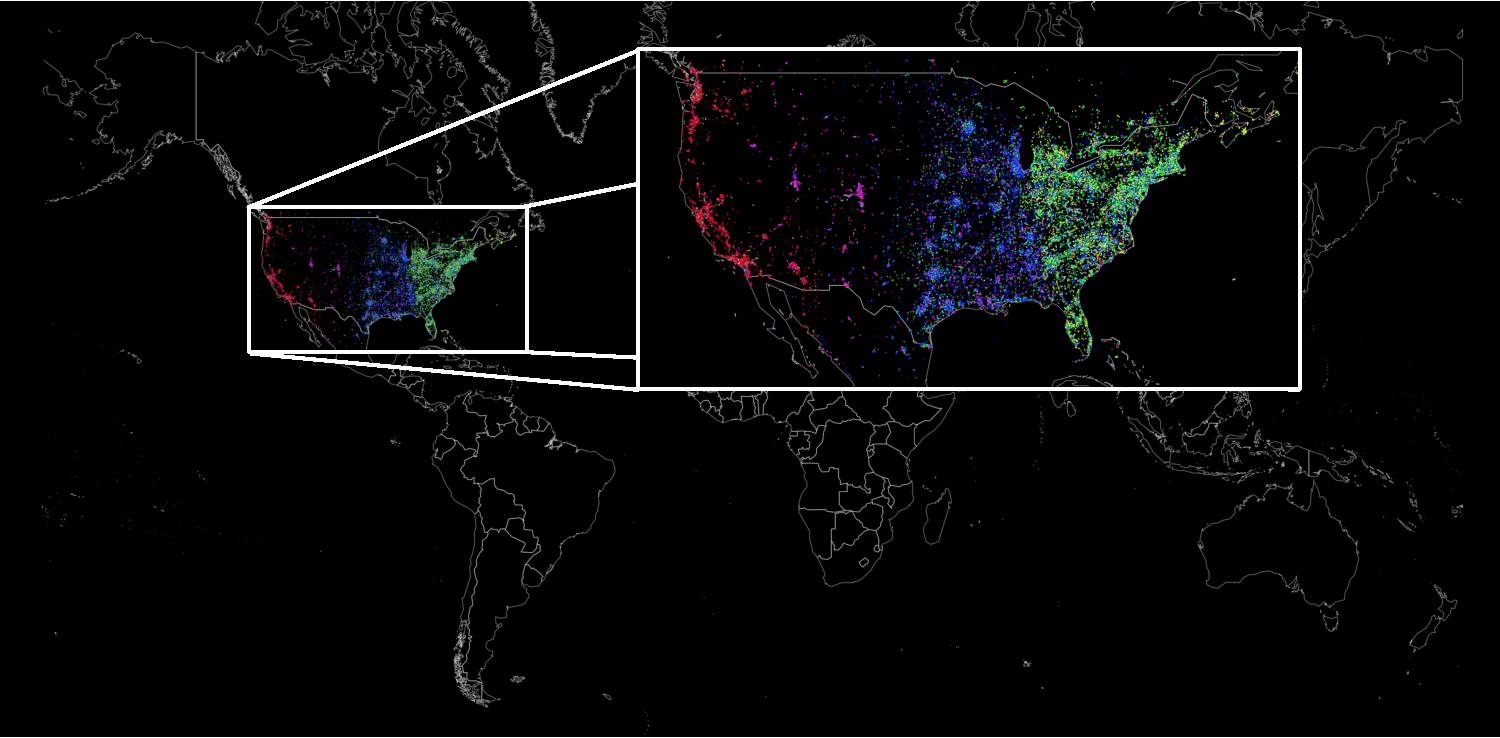
\includegraphics[scale=0.5]{usTimezones.pdf}
							\caption{Tweets, abhängig der Zeitzone eingefärbt}
							\label{img:usTimezones}
						\end{center}
					\end{figure}	

					Lediglich die dünn besiedelte Region der Mountain Time kann nur an einigen Ballungszentren erkannt werden. 
					Grundsätzlich scheint der Großteil der Angaben aber korrekt zu sein.

					Ist ein Toponym doppel- oder mehrdeutig kann nicht entschieden werden welches geografische Objekt zugeordnet werden soll.
					Liegen die beiden geografischen Objekte allerdings in zwei unterschiedlichen Zeitzonen und der Nutzer hat die Nutzer-Zeitzone korrekt angegeben kann die Doppeldeutigkeit aufgelöst werden.
					Voraussetzung hierfür ist natürlich, dass die geografischen Objekte in zwei unterschiedlichen Zeitzonen liegen und die Nutzer-Zeitzone angegeben ist.

				\textit{Hinzufügen der Nutzer-Zeitzone}

					An die Referenzwerte, die aus dem Nutzer-Standort erzeugt wurden soll nun die Zeitzone angehängt werden.
					Jeder Referenzwert soll einmal mit und einmal ohne Zeitzone existieren. 
					Damit wird garantiert, dass eingelernte Referenzwerte, die eine falsche Zeitzone aufweisen, trotzdem berücksichtigt werden können. 

					Um die Nutzer-Zeitzone von den aus dem Nutzer-Standort generierten Elementen unterscheiden zu können, wird die Nutzer-Zeitzone kursiv geschrieben.
					Auch hier wird die Liste weiter eingeschränkt und es werden lediglich noch zwei Beispiele betrachtet.
					
					\begin{table}[h]
					\centering
					\caption{Hinzufügen der Zeitzone}
					\label{tab:ngramsWithTZ}
					\begin{tabular}{|l|l|}
					\hline
					  & \textbf{Referenzwerte}                                                                     \\ \hline
					1 & \textless Los+Angeles\textgreater\textless USA\textgreater                                   \\ \hline
					2 & \textless Los+Angeles\textgreater                                                           \\ \hline
					3 & \textless USA\textgreater                                                                   \\ \hline
					4 & \textless Los+Angeles\textgreater\textless USA\textgreater\textless \textit{Pacific+Times}\textgreater \\ \hline
					5 & \textless Los+Angeles\textgreater\textless \textit{Pacific+Times}\textgreater               \\ \hline
					6 & \textless USA\textgreater\textless \textit{Pacific+Times}\textgreater                       \\ \hline
					7 & \textless York\textgreater                                                                  \\ \hline
					8 & \textless York\textgreater\textless \textit{London+Time}\textgreater                        \\ \hline
					\end{tabular}
					\end{table}

					Ein Beispiel für eine Auflösung der Doppeldeutigkeit ist in Tabelle \ref{tab:ngramsWithTZ} für das Token \textless York\textgreater  angegeben.
					Zum einen existiert "'York"' in England zum anderen in den USA.  
					Mit Hilfe der zusätzlichen Zeitzone können geografische Objekte, wenn sie in verschiedenen Zeitzonen liegen, unterschieden werden.

		\subsection{Bestimmung der absoluten Häufigkeiten der Referenzwerte}

			Es werden nun die absoluten Häufigkeiten der Referenzwerte bestimmt.
			Dabei werden die Vorkommen der Referenzwerte an einer geografischen Position gezählt.

			Jedes oben ermittelte N-Gramm und die Kombination aus N-Gramm und Zeitzone werden als einzelne Referenzwerte betrachtet. 
			Jedem Referenzwert werden die geografischen Koordinaten des Tweets zugeordnet, aus dem der Referenzwert erzeugt wurde.
			Zur Verdeutlichung ist in Tabelle \ref{tab:bspWerteAusEinemTweet} das Ergebnis der oben genannten Schritte an einem Beispiel dargestellt. 

				\begin{table}[h]
				\begin{tabular}{|l|l|l|}
				\hline
				\textbf{}         & Nutzer-Standortfeld:                                                                       & love Los Angeles                                                \\ \cline{2-3} 
				\textbf{Ursprung} & Nutzer-Zeitzone                                                                            & Pacific Time                                                    \\ \cline{2-3} 
				\textbf{}         & Geografische Koordinaten                                                                   & (33.78,118.29)                                                  \\ \hline
				                  & \multicolumn{1}{c|}{\textit{\textbf{Referenzwert}}}                                        & \multicolumn{1}{c|}{\textit{\textbf{geografische Koordinaten}}} \\ \hline
				1                 & \textless Los+Angeles\textgreater\textless love\textgreater                                  & (33.78, 118.29)                                                 \\ \hline
				2                 & \textless Los+Angeles\textgreater                                                           & (33.78, 118.29)                                                 \\ \hline
				3                 & \textless love\textgreater                                                                  & (33.78, 118.29)                                                 \\ \hline
				5                 & \textless Los+Angeles\textgreater\textless love\textgreater\textless Pacific+Time\textgreater & (33.78, 118.29)                                                 \\ \hline
				\textit{6}        & \textless Los+Angeles\textgreater\textless Pacific+Time\textgreater                          & \textit{(33.78, 118.29)}                                        \\ \hline
				7                 & \textless Los+Angeles\textgreater\textless love\textgreater\textless Pacific+Time\textgreater & (33.78, 118.29)                                                 \\ \hline
				\end{tabular}
				\end{table}


			Jeder Tweet aus den Trainingsdatensätzen wird in dieser Weise verarbeitet. 
			Es liegt damit eine Menge an Referenzwerten mit zugehörigen geografischen Koordinaten vor.

			Mit Hilfe dieser Daten wird nun die Georeferenz-Basis aufgebaut. 
			Für jedes Tupel wird in der vorgestellten Struktur der Georeferenz-Basis (siehe Tabelle \ref{tab:strukturMitHierarchie1}) ein Datensatz angelegt und mit einem Wert von 1 für die absolute Häufigkeit initialisiert. 
			Stimmt sowohl der Referenzwert als auch die geografische Position mit einem vorhandenen Datensatz überein, wird die absolute Häufigkeit für dieses Tupel inkrementiert.
			In dieser Art werden alle erzeugten Referenzwerte und geografischen Postionen verglichen und die Anzahl der Vorkommen an einer geografischen Position erfasst.

			Die geografischen Koordinaten eines Tweets sind für diese Art der quantitativen Erfassung allerdings zu genau. 
			Der Längen- und Breitengrad wird meistens mit Hilfe von GPS-Modulen mobiler Endgeräte, wie Smartphones, erfasst.
			Diese geben eine Position oft auf wenige Meter genau an.
			Das bedeutet, zwei Tweets die wenige Meter voneinander abgesetzt wurden haben in der Regel unterschiedliche Werte für den Längen- und Breitengrad.
			Dies kann für die Bestimmung der Häufigkeiten problematisch sein, da die Werte des Längen- und Breitengrades in der Regel nicht exakt übereinstimmen.

		\subsection{Zuordnung der nächstgelegenen Stadt mit Hilfe von Voronoi-Regionen} 

			Um die geografischen Positionen der Referenzwerte vergleichbar zu machen, wird jeder Referenzwert auf die geografischen Koordinaten der nächstgelegenen Stadt abgebildet.
			Dies wird mit Hilfe von Voronoi-Diagrammen umgesetzt.

			In einem Voronoi-Diagramm ist eine Ebene und eine Menge an Punkten derart zerlegt, dass jedem Punkt eine Region zugeordnet wird, die sogenannten Voronoi-Regionen.
			In jeder dieser Region liegt dabei exakt ein Punkt.  

			Sei eine Menge von Punkten $Z = {z_1,z_2,...,z_n}$ auf einer Ebene verteilt.
			Eine Voronoi-Region $V^i$ zu einem Punkt $z_i$ beinhaltet dann alle Punkte $P^i={p_1,p_2,...,p_n}$ die näher an $z_i$ liegen als an allen anderen Punkten $Z_j={z_j in Z|z_j!=z_i}$.
			Alle Voronoi-Regionen zu allen Punkten in Z bilden ein Voronoi-Diagramm.

			Dieses Konzept kann zur Bestimmung der nächstgelegenen Stadt verwendet werden. 
			Die geografischen Positionen der Städte bilden dabei die Menge der Punkte $Z$ zur Bestimmung der Vornoi-Regionen.
			Zu diesen geografischen Koordinaten werden nun die Voronoi-Regionen erzeugt. 
			Anhand der Voronoi-Region in der ein Punkt $p$ liegt kann nun bestimmt werden welche Stadt $z_i$ am nächsten zu $p$ liegt.

			Jeder Punkt auf dem Globus kann so einer Stadt und deren geografischen Position zugeordnet werden.
			Dadurch wird der Globus auf Städteebene in geografische Regionen eingeteilt.
			In Abbildung \ref{img:voronoi} ist ein Voronoi-Diagramm einiger deutscher Städte dargestellt.

			\begin{figure}[h!]
				\begin{center}
				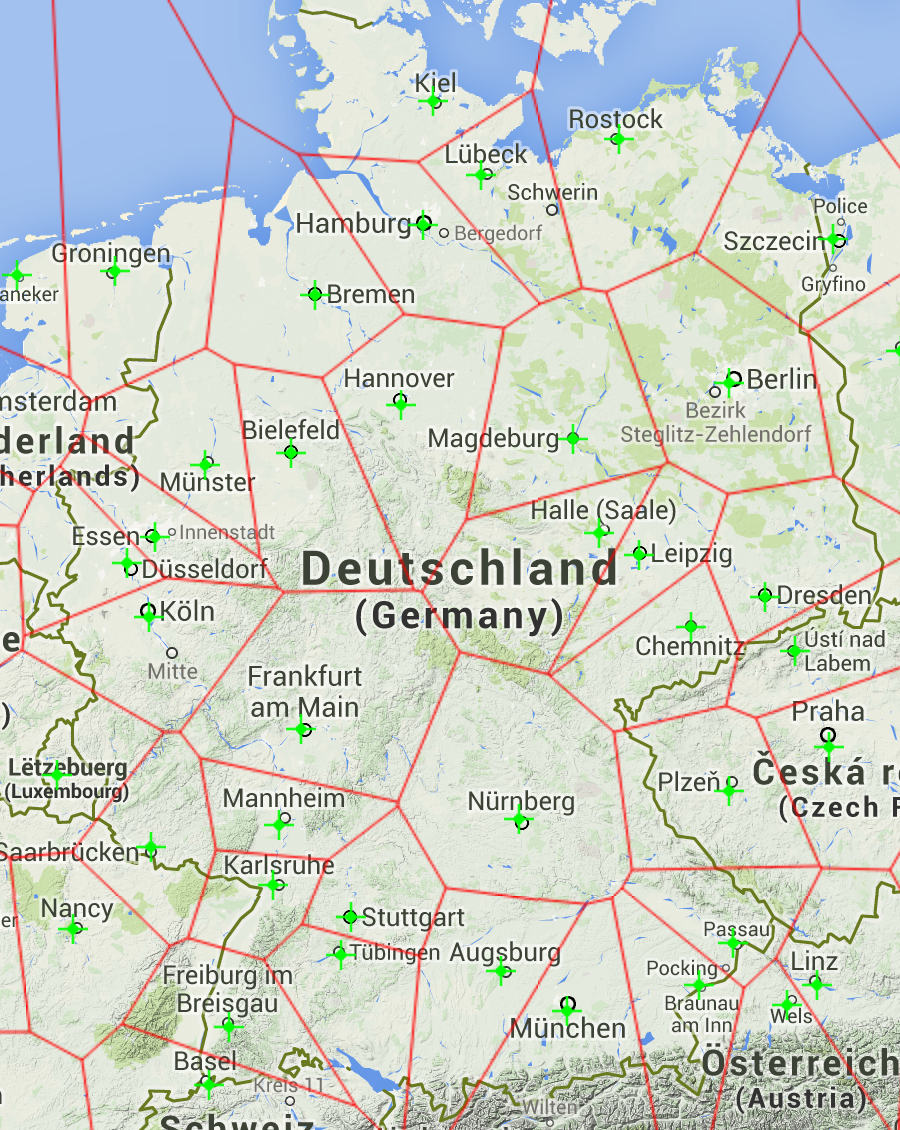
\includegraphics[scale=0.5]{voronoi.png}
				\caption{Beispiel eines Vornoi-Diagramm für einige deutsche Städte}
				\label{img:voronoi}
				\end{center}
			\end{figure}	

			% Quelle: http://lpetrich.org/Science/GeometryDemo/GeometryDemo_GMap.html

			In dicht besiedelten Gebieten können viele kleine Städte vorhanden sein. 
			Damit wäre die Positionsangabe wiederum zu genau.
			Es werden deshalb nur Städte verwendet deren Einwohnerzahl 15000 überschreitet.
			Jeder Referenzwert wird also der nächstgelegenen Stadt mit mehr als 15000 Einwohnern zugeordnet.
			In Ballungsräumen sind damit mehr Städte zu erwarten, womit kleinere Voronoi-Regionen entstehen.
			Dadurch nimmt die Genauigkeit zu.
			In diesen Gegenden sind allerdings auch mehr Tweets zu erwarten, womit pro Voronoi-Region für die spätere Auswertung ausreichend Referenzwerte vorhanden sind. 
			In ländlichen Gebieten sind hingegen viele kleine Orte und nur wenigen große Städte zu erwarten diese werden dadurch in größere Voronoi-Regionen eingeteilt.
			Es sind allerdings auch weniger Tweets zu erwarten. 
			Durch das größere Einzugsgebiet kann dennoch eine ausreichende Anzahl an Referenzwerten einer Stadt zugeordnet werden. 

			Die geografischen Koordinaten der Referenzwerte werden dadurch auf eine definierte Menge geografischer Koordinaten abgebildet. 
			Jeder dieser geografischen Koordinaten ist eine Stadt zugeordnet.
			Dies kann als Übergang einer kontinuierlichen Darstellung durch geografische Koordinaten zu einer diskreten Darstellung durch Städte angesehen werden. 
			Durch die Teilmengenbeziehung ist es nun nicht mehr nötig, die geografischen Regionen der anderen Hierarchieebenen zu bestimmen. 
			Diese werden durch die Stadt implizit mitbestimmt.
			
			\textit{Bewertung des Verfahrens zur Bestimmung der nächstgelegenen Stadt}

				Durch die Zuordnung zu Städten, die hier eine exakte geografische Position in Form geografischer Koordinaten aufweisen, entstehen gewisse Ungenauigkeiten.
				Um das Verfahren zu bewerten wurden die Distanzen, welche zwischen der tatsächlichen Position eines Tweets und der zugeordneten Stadt liegen, protokolliert. 
				Dies spiegelt den Fehler des Zuordnungsverfahrens wieder.

				In Tabelle \ref{tab:distances} sind die Ergebnisse dargestellt.
				Es wurden 383222 Tweets untersucht.
				Im Median liegt die Fehlerdistanz zwischen der tatsächlichen Position und der zugeordneten Stadt bei 3,5 Kilometern.
				Über die Quantile können die Fehlerdistanzen noch genauer untersucht werden.
				Das 0.25 Quantil sagt aus, dass 25\% aller Fehlerdistanzen unter 1,7 Kilometern liegen.
				Der Wert für das 0.95 Quantil liegt bei 24,1 Kilometer, 95\% der Tweets waren näher als 24,1 Kilometer an der zugeordneten Stadt. 
				Dies ist ausreichend genau. 

					\begin{table}[h]
					\centering
					\caption{Fehlerdistanzen zwischen Tweet Ursprung und zugeordneter Stadt (in km)}
					\label{tab:distances}
					\begin{tabular}{|l|l|}
					\hline
					Durchschnitt & 7      \\ \hline
					Median       & 3.5    \\ \hline
					0.25 Quantil & 1.7    \\ \hline
					0.75 Quantil & 6.9    \\ \hline
					0.85 Quantil & 10     \\ \hline
					0.95 Quantil & 24.1   \\ \hline
					0.98 Quantil & 44.2   \\ \hline
					Größte Distanz      & 3424.5 \\ \hline
					Kleinste Distanz     & 0     \\ \hline
					\end{tabular}
					\end{table}

			\textit{Grenzen des Verfahrens zur Bestimmung der nächstgelegenen Stadt}

				Es ist zu beachten, dass durch die Erzeugung der Vornoi-Regionen Ländergrenzen nur approximiert werden können. 
				Voronoi-Regionen zu Städten die in der Nähe einer Landesgrenze liegen können über die Landesgrenzen hinausgehen. 
				Damit werden geografische Positionen unter Umständen dem falschen Land zugeordnet.
				Auch dies ist in Abbildung \ref{img:voronoi} an den Landesgrenzen zu erkennen. 
				Umso größer allerdings die Anzahl der Städte ist die betrachtet wird, umso genauer wird die Approximation. 

	\section{Geolokalisierung: Auflösen des Nutzer-Standortes mit Hilfe der Georeferenz-Basis} \label{sec:AufloesenDesNutzerStandortes} 

		Es soll nun das Verfahren zur Geolokalisierung eines Tweets vorgestellt werden.
		Dabei dient die Georeferenz-Basis und die in ihr abgelegten Referenzwerte als Basis für die Zuweisung einer Georeferenz.

		Zunächst werden aus dem Nutzer-Standort und der Nutzer-Zeitzone potenzielle geografische Indikatoren erzeugt.
		Dies geschieht analog zur Erzeugung von Referenzwerten beim einlernen der Georeferenz-Basis.
		Es werden also dieselben Vorverarbeitungsschritte für den Nutzer-Standort und die Nutzer-Zeitzone durchgeführt.
		Daraus resultiert eine Menge potenzieller geografischer Indikatoren.
		Die Werte der potenziellen geografischen Indikatoren werden nun in der Georeferenz-Basis nachgeschlagen. 
		Dabei werden alle Datensätze deren Referenzwerte mit den potenziellen geografischen Indikatoren korrespondieren zurückgegeben.
		Auf diesen Datensätzen erfolgt die weitere Verarbeitung und Bestimmung der wahrscheinlichsten Georeferenz.
		
		Es liegt nun eine Menge an Datensätzen aus der Georeferenz-Basis vor.
		Die Referenzwerte entsprechen dabei den potenziellen geografischen Indikatoren.
		Die absoluten und relativen Häufigkeiten werden für jeden Referenzwert separat analysiert.
		Das Ziel der Analyse ist es, die wahrscheinlichste Georeferenz zu ermitteln.

		In Abbildung \ref{img:ablaufGeolok} ist der gesamte Ablauf an einem Beispiel dargestellt.
		In den folgenden Abschnitten soll nun die Analyse genauer betrachtet werden.

			\begin{figure} 
			\begin{center}
						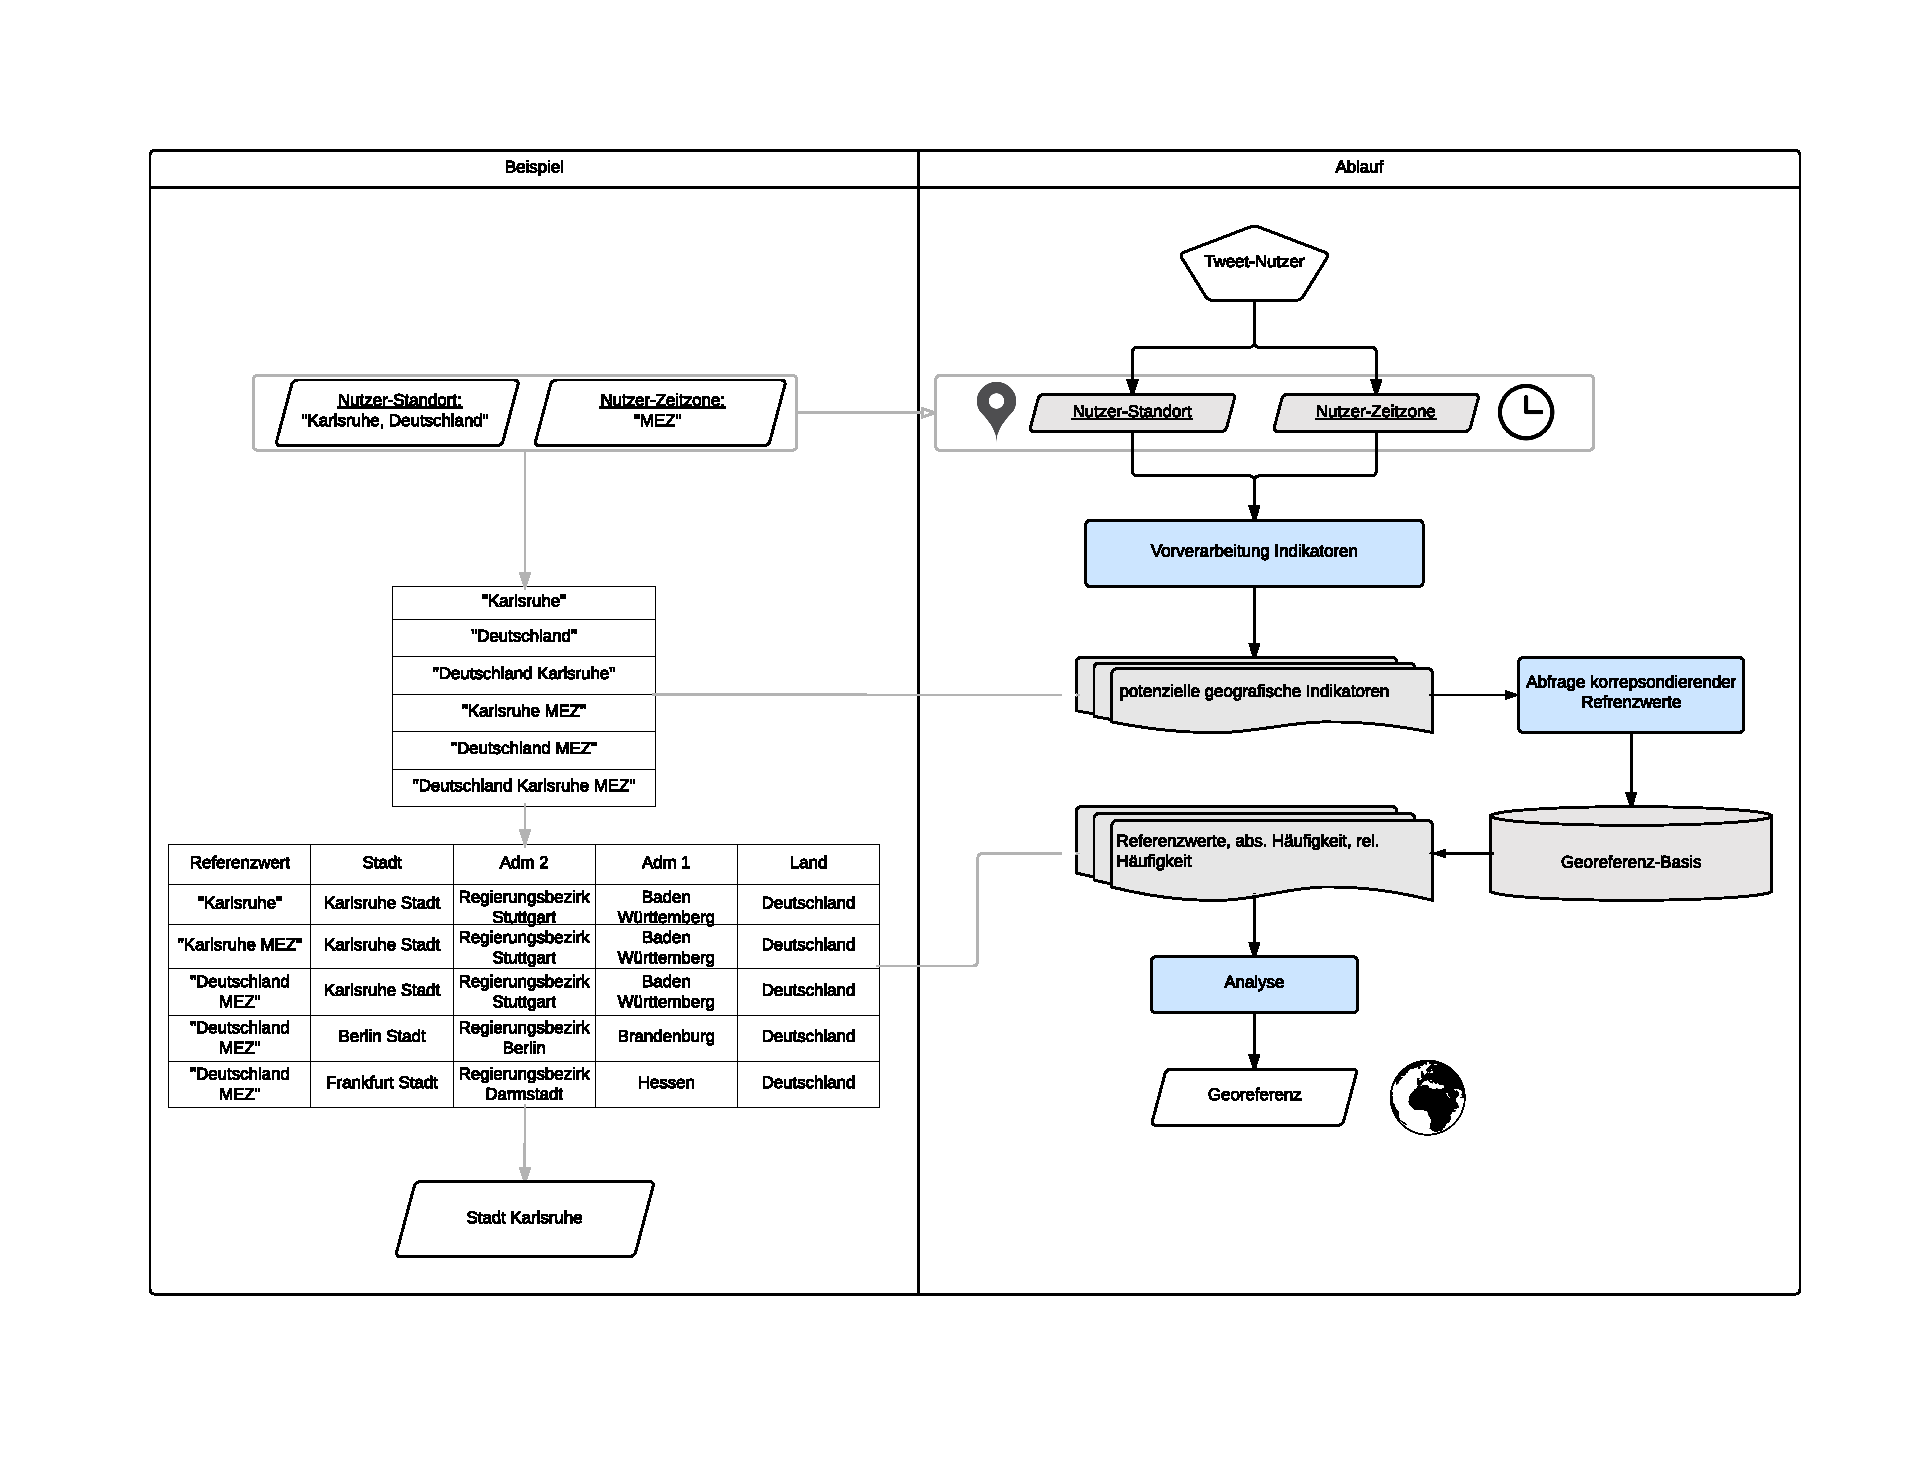
\includegraphics[scale=0.5]{geolokalisierungAllg.pdf}
						\caption{Ablauf der Geolokalisierung mit Beispiel}
						\label{img:ablaufGeolok}
					\end{center}
			\end{figure}	

		In diesem Abschnitt wird ein Verfahren vorgestellt, welches es ermöglicht einem Tweet mit Hilfe der Georeferenz-Basis eine Georeferenz zuzuordnen. 


		In der Georeferenz-Basis sind alle Werte aus den Nutzer-Standorten der Lerndatensätze enthalten.
		Es sind also auch Referenzwerte vorhanden die keinen geografischen Bezug haben.
		
		Es ist die Frage zu beantworten: \\ Wie kann bestimmt werden ob ein Referenzwert geografischen Bezug hat oder nicht? \\
		Oder: \\ Wie kann vermieden werden, dass ein Referenzwert, der keinen geografischen Bezug hat, zur Geolokalisierung genutzt wird?
		
		Dies ist wichtig, denn durch die Referenzwerte wird einem geografischen Indikator eine Georeferenz zugewiesen. 
		Wird einem geografischen Indikator durch einen Referenzwert ohne geografischen Bezug eine Georeferenz zugewiesen ist diese mit hoher Wahrscheinlichkeit fehlerhaft.
		Dies wiederum führt zu schlechten und unzuverlässigen Ergebnissen.
		Es muss also ein Verfahren gefunden werden um zu entscheiden ob die Referenzwerte einen geografischen Bezug haben oder nicht.

		Es ist zu beachten, dass die Vorverarbeitung keine Aussage zum geografischen Bezug macht, sondern vielmehr die Referenzwerte aus den Nutzer-Standorten extrahiert. 
		Dies soll sicherstellen, das möglichst viele Informationen aus den Nutzer-Standorten gezogen werden können und insbesondere keine Informationen verloren gehen.  
		
		Um zu entscheiden ob ein Referenzwert geografischen Bezug hat oder nicht wird die absolute Häufigkeit verwendet.
		Die absoluten Häufigkeiten geben an wie oft ein Referenzwert in einer bestimmten Region, zunächst in der Voronoi-Region der entsprechenden Stadt, vorkommt.			 
		Daraus kann nun ein geografischer Bezug abgeleitet werden.

		In Kapitel \ref{sec:einlernen} wurde ein Verfahren zum einlernen der Georeferenz-Basis vorgestellt. 
		Im darauffolgenden Kapitel \ref{sec:geografischerBezug} wurde eine Möglichkeit vorgestellt wie der geografische Bezug der Referenzwerte untersucht werden kann.
		Dies soll hier genutzt werden um eine Georeferenz zu bestimmen. 

		

		Grundsätzliche Idee des auflösens mit absoluten Häufigkeiten
		Hier Idee skizzieren. 
		Schwellwert für den absoluten Häufigkeitswert zur Justierung der Konfidenzen.

		\subsection{Geolokalsierung: Auflösen des Nutzer-Standortes basierend auf absoluten Häufigkeiten} 

			\todo{chap: LsgAnsatz sec: Auflösen subsec: abs. Hauf. Komplette Einführung + Ablauf + Auswertung} 

			\subsubsection{Ablauf}

			\subsubsection{Auswertung}  

				\textit{Die absolute Häufigkeit als Hinweis auf geografischen Bezug zu Städten} 
				
				Eine hohe absolute Häufigkeit kann ein Hinweis auf den geografischen Bezug eines Referenzwertes darstellen. 
				Aufgrund der Eigenschaften des Nutzer-Standorts ist anzunehmen, dass in der Voronoi-Region einer Stadt der Name der zugehörigen Stadt häufig vorkommt.
				Dadurch kann eine Relevanz des Referenzwertes zu einer Stadt abgeleitet werden. 
				Tritt der Referenzwert nicht häufig auf, so ist er von nur wenigen Nutzern als Nutzer-Standort in einer Stadt angegeben worden und somit für die Stadt nicht relevant.
				In Abbildung \ref{img:ulIstanbulWalesZoom} sind die Tweets in denen "'Istanbul"' im Nutzer-Standort vorkommt aufgetragen.
				Es ist deutlich eine Häufung um die Stadt Istanbul zu erkennen. 
				Werden die Tweets rund um Istanbul nun auf die Stadt Istanbul abgebildet, wird die Kombination aus dem Referenzwert "'Istanbul"' und der Georeferenz Istanbul sehr häufig vorkommen.
				In den Nutzer-Standorten der Tweets rund um Istanbul taucht "'Istanbul"' tatsächlich 972 mal auf.
				Damit kann eine Gewisse Relevanz für den Referenzwert "'Istanbul"' zur Stadt Istanbul abgeleitet werden.

				\begin{figure}[!ht]
						\begin{center}
							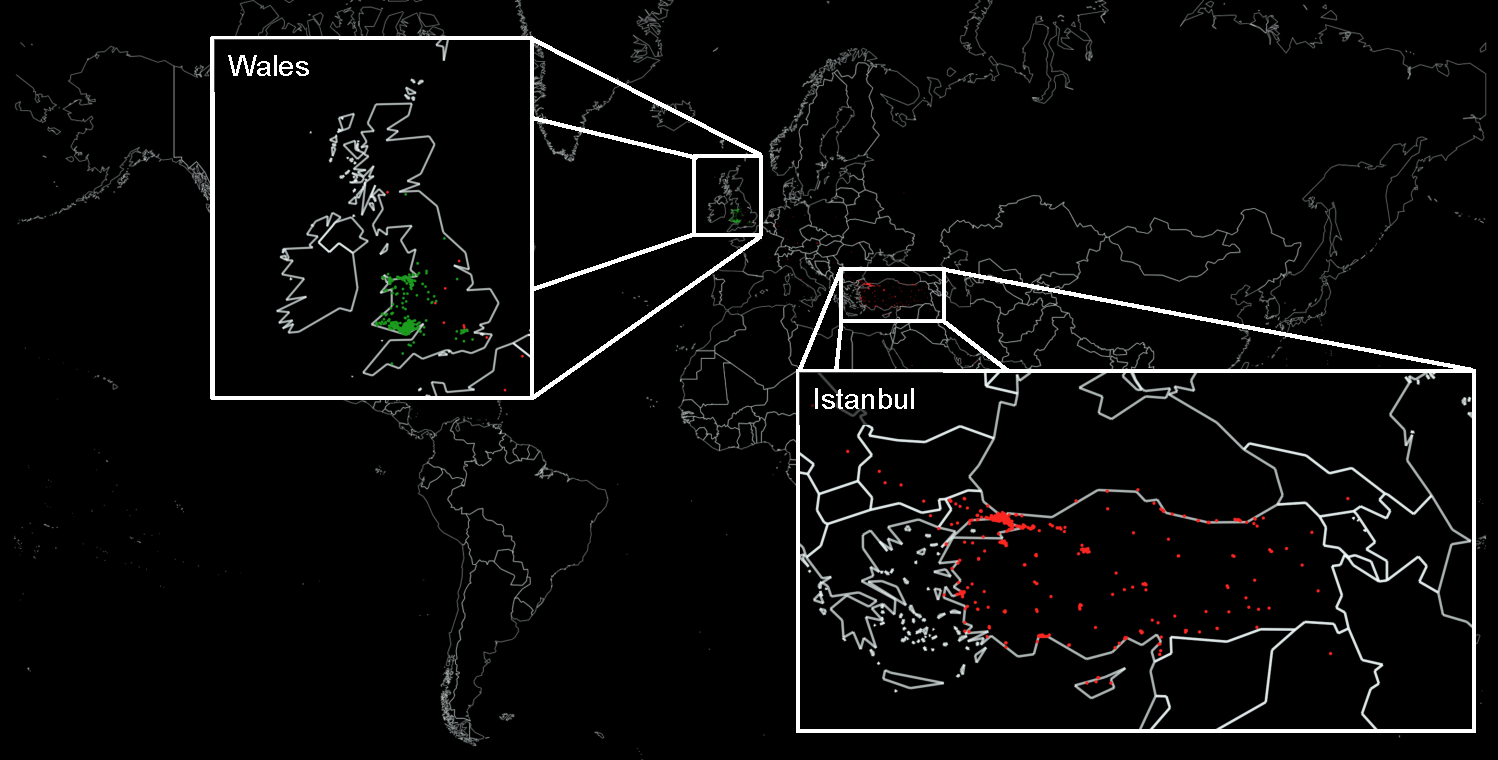
\includegraphics[scale=0.5]{ulIstanbulWalesZoom.pdf}
							\caption{}
							\label{img:ulIstanbulWalesZoom}
						\end{center}
				\end{figure}	

				Es kann also ein Schwellwert für die Häufigkeit eingeführt werden um Referenzwerte mit geografischem Bezug zu identifizieren.
				Allerdings garantiert die absolute Häufigkeit noch nicht, dass ein Referenzwert einen geografischen Bezug hat. 
				Es können auch Werte an einem bestimmten Ort häufig vorkommen, die keinen geografischen Bezug haben.
				Um dies erkennen zu können muss ein weiterer Wert berechnet werden.

		\subsection{Probleme bei der ausschließlichen Betrachtung der absoluten Häufigkeiten} 

			Betrachtet man die absoluten Häufigkeiten isoliert voneinander wird die Verteilung des Referenzwertes außer acht gelassen. 
			Ein Referenzwert kann eine gleichmäßige Verteilung über mehrere Städte aufweisen.
			Das bedeutet, der Referenzwert wird in vielen unterschiedlichen Städten benutzt. 
			Es können trotzdem Häufungen in Städten auftreten.
			Diese können sogar über einem gewählten Schwellwert für die absolute Häufigkeit liegen.
			Die Häufung kann jedoch relativ gesehen sehr gering sein.
			Dies ist ein Hinweis darauf das der Referenzwert keinen geografischen Bezug hat.
			Die relative Häufung sagt hier aus, das ein Referenzwert sehr verteilt auftritt. 
			Es ist also wichtig nicht nur die absoluten Häufigkeiten, sondern auch die relativen Häufigkeiten der Referenzwerte zu berücksichtigen.

			Problem am Beispiel und mit Daten.

			Einbeziehung der relativen Häufigkeiten. 
			Aufgrund von Beispielbetrachtung The und La Plata. Absolut betrachtet.


			"'La Plata"' tritt rund um die Stadt La Plata in Argentien 91 mal auf.
			Der Referenzwert "'La Plata"' hat offensichtlich einen geografischen Bezug zu einer Stadt. 

			Obwohl "'the"' keinen offensichtlichen geografischen Bezug hat ist die absolute Häufigkeit von 91 Vorkommen in Jakarta hoch.
			Der Schwellwert könnte nun aufgrund der Erfahrung mit dem Referenzwert "'La Plata"' auf 90 angesetzt werden.
			Dann würde davon ausgegangen werden, dass der Referenzwert "'the"' einen geografischen Bezug hat.
			Betrachtet man allerdings die Abbildung \ref{img:ULThe} fällt auf, dass Tweets mit dem Wert "'the"' im Nutzer-Standort sehr verteilt auf dem Globus auftreten.
			Im Gegensatz dazu tritt "'La Plata"' in den Nutzer-Standorten sehr konzentriert auf.
			In Abbildung \ref{img:ULlaPlata} wird die Verteilung von Tweets deren Verfasser "'La Plata"' im Nutzer-Standort enthalten dargestellt. 
			Es ist deutlich eine Häufung um die Stadt La Plata in Argentien zu erkennen, weltweit tritt der Referenzwert aber sehr selten auf.
			\begin{figure} 
				\begin{center}
					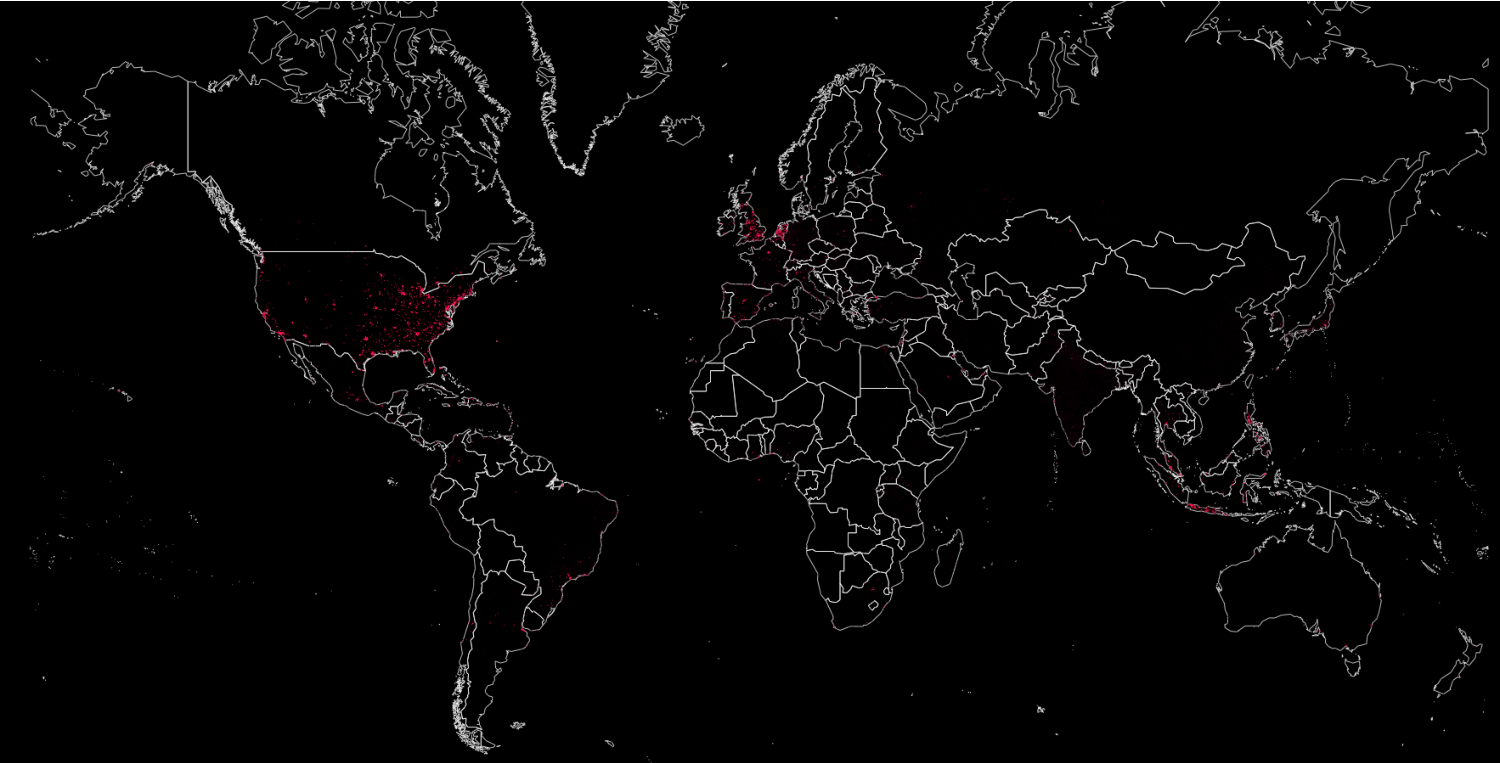
\includegraphics[scale=0.6]{ulTheG.pdf}
					\caption{Tweets mit Nutzer-Standort "'The"'}
					\label{img:ULThe}
					\end{center}
				\end{figure}
			\begin{figure}
			\begin{center}
					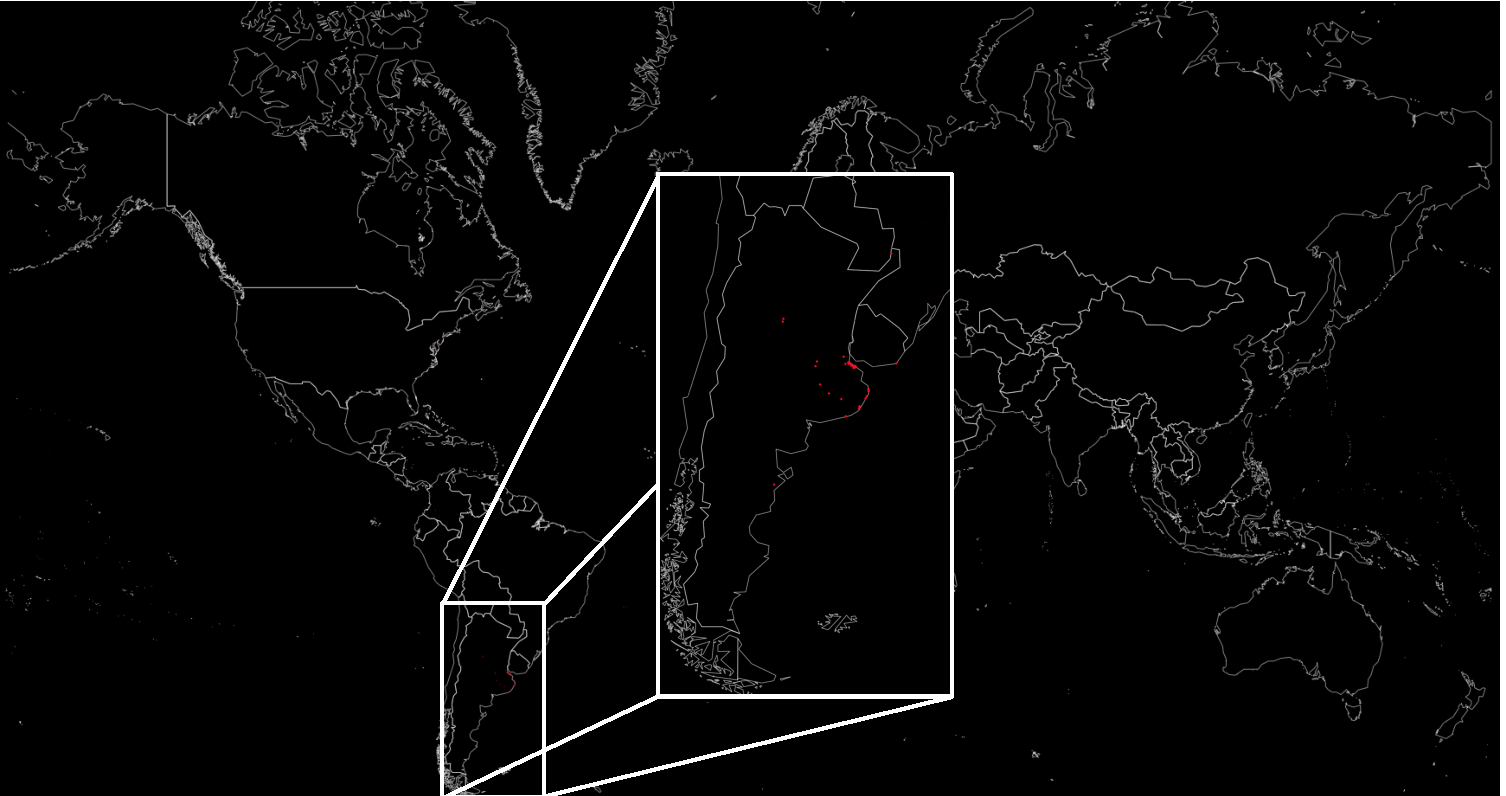
\includegraphics[scale=0.5]{ulLaPlataG.pdf}
					\caption{Tweets mit Nutzer-Standort "'La Plata"'}
					\label{img:ULlaPlata}
				\end{center}
			\end{figure}		

		\subsection{Auflösen des Nutzer-Standortes basierend auf absoluten und relativen Häufigkeiten} 

			Idee skizzieren
			\todo{chap: LsgAnsatz sec: Auflösen subsec: abs. Hauf. Komplette Einführung + Beispiel überarbeiten} 

			\textit{Berechnung der relativen Häufigkeiten}  

				Um die relativen Häufigkeiten zu berechnen soll das Vorkommen eines Referenzwertes in einer Stadt, durch die Gesamtanzahl der Vorkommen des Referenzwertes geteilt werden.
				Damit erhält man den prozentualen Anteil der auf eine Stadt entfallenden Vorkommen eines Referenzwertes.
				Als Basis für diese Berechnung dienen die absoluten Häufigkeiten.

				Sei $(r_i,c_j)$ ein Datensatz der Georeferenz-Basis mit Referenzwert $r_i$ und Georeferenz $c_i$.
				Des weiteren liefert $H(r_{i},c_{j})$ die absolute Häufigkeit zu einem Referenzwert $r_i$ und einer Georefrenz $c_i$. 

				Damit kann die relative Häufigkeit $rel_{(r_i,c_j)}$ für jede Kombination $(r_i,c_j)$ durch die folgende Formel berechnet werden. 
				$n_c$ ist dabei die Anzahl aller Georeferenzen.

				\begin{equation}
					d_{r_i,c_j}=\frac{H(r_i,c_j)}{\sum^{n_c}_{j=0}{H(r_i,c_j)}}
				\end{equation}	

			\subsubsection{Ablauf}

			\subsubsection{Lösung des Beispielproblems von oben}

				Berechnet man nun die relativen Häufigkeiten kann dies abgebildet werden.
				In Tabelle \ref{tab:the} sind die zugeordneten Städte, die absoluten Häufigkeiten und die berechneten relativen Häufigkeiten für die Vorkommen des Wortes "'the"' aufgetragen. 
				Die Einträge sind absteigend nach dem Wert der relativen Häufigkeit sortiert.
				In Tabelle \ref{tab:the} werden nur die vier ersten Einträge dargestellt.  
				Insgesamt kam das Wort "'the"' in 2824 verschiedenen Städten vor.
				Dabei wurde es insgesamt 5764 mal verwendet. 
				Trotz der hohen absoluten Häufigkeit in Jakarta liegt die relative Häufigkeit bei lediglich 1,6\%.
				Aus den relativen Häufigkeiten lässt sich nun die, in Abbildung \ref{img:ULThe} vermutete, globale Verteilung ablesen.


				\begin{table}[h]
				\centering
				\caption{"'the"'}
				\label{tab:the}
				\begin{tabular}{|l|l|l|}
				\hline
				Stadt             & abs. Häufigkeit & rel. Häufigkeit in \% \\ \hline \hline
				Jakarta           & 91              & 1,6                       \\ \hline
				Singapore         & 27              & 0,5                       \\ \hline
				Bekasi            & 25              & 0,4                       \\ \hline
				Philadelphia      & 23              & 0,4                       \\ \hline
				... & ... & ... \\ \hline
				\end{tabular}
				\end{table}

				Die Verteilung erklärt sich dadurch, dass das Wort "'the"' im englischen sehr häufig auftritt.
				Englisch ist die internationale Verkehrssprache und wird dementsprechend global und sehr häufig verwendet.
				Dies spiegelt sich in der Verteilung der vorkommen auf dem Globus wieder.
				Die Häufung um Jakarta kann teilweise damit erklärt werden, dass sehr viele Tweets die in und um Jakarta abgesetzt werden eine Angabe von Längen- und Breitengrad aufweisen. 

				In Tabelle \ref{tab:laPlata} wird dieselbe Auswertung für "'La Plata"' dargestellt. 
				"'La Plata"' ist insgesamt 129 mal in 23 verschiedenen Städten aufgetaucht. 
				In der Stadt La Plata, in Argentien, kam es 91 mal vor.
				Dies entspricht einer relativen Häufigkeit von 70,5\%.

				\begin{table}[h]
				\centering
				\caption{"'La Plata"'}
				\label{tab:laPlata}
				\begin{tabular}{|l|l|l|}
				\hline
				Stadt            & abs. Häufigkeit & rel. Häufigkeit in \% \\ \hline \hline
				La Plata         & 91              & 70,5                      \\ \hline
				Villa Gesell     & 9               & 7,0                       \\ \hline
				Mar del Plata    & 5               & 3,9                       \\ \hline
				Quilmes          & 3               & 2,3                       \\ \hline
				... & ... & ... \\ \hline
				\end{tabular}
				\end{table}

				"'La Plata"' taucht erwartungsgemäß am häufigsten rund um die Stadt La Plata auf.  

				Es lässt sich also anhand der relativen Häufigkeiten ein geografischer Bezug des Referenzwertes nachweisen.
				Damit kann man zunächst bestimmen ob ein Referenzwert geografischen Bezug hat oder nicht.
				Die relativen Häufigkeiten können nach dem einlernen der Referenzwerte berechnet und in der Georeferenz-Basis hinterlegt werden.
				Mit Hilfe eines Schwellwertes für die relativen Häufigkeiten, kann nun bestimmt werden wann ein Referenzwert geografischen Bezug hat.

				Aber auch die ausschließliche Betrachtung der relativen Häufigkeiten reicht nicht aus um die geografische Relevanz nachzuweisen.
				Da die relativen Häufigkeiten basierend auf den Vorkommen des Referenzwertes berechnet werden sagen diese wiederum nichts über die absoluten Häufigkeit aus. 
				Kommt ein Referenzwert zwei mal in zwei verschiedenen Städten vor, liegen die jeweiligen relativen Häufigkeiten bei 50\%.
				Dies ist ein hoher Wert.
				Da der Referenzwert aber nur einmal vorkam, ist es sehr unwahrscheinlich das er einen geografischen Bezug hat.  

		\subsection{Einführung von Schwellwerten für die absolute und relative Häufigkeit zur Justierung der Ergebnisse}  

			\todo{chap: LsgAnsatz sec: Auflösen subsec: Schwellwerte für abs. und rel. einführen komplett schreiben} 

	\section{Ausnutzen der geografischen Hierarchie zur Verbesserung der Ergebnisse} \label{sec:ausnutzenDerGeografischenHierarchie}

		\todo{chap: LsgAnsatz sec: Ausnutzen Hierarch subsec: Idee skizzieren und Splitten -> mergen} 
		Idee skizzieren

		\textit{Geografischer Bezug zu Verwaltungseinheiten und Ländern} 

			Beim einlernen der Georeferenz-Basis werden durch die absoluten Häufigkeiten die Vorkommen pro Stadt gespeichert.
			Mit den daraus errechneten relativen Häufigkeiten kann nicht entschieden werden, ob für den Referenzwert eine globale Verteilung vorliegt oder ob der Referenzwert unter Umständen nur regional begrenzt, zum Beispiel in einem Land, auftritt.
			Für Referenzwerte die ein Land oder eine Verwaltungseinheit bezeichnen ist auf Städteebene eine geringe relative Häufigkeit zu erwarten.
			Diese Referenzwerte treten in einer größeren geografischen Region als der Voronoi-Region einer Stadt auf.
			Sie sind somit über mehrere Städte verteilt und werden auf Stadtebene einer geringe relative Häufigkeit aufweisen.
			Es ist beispielsweise zu erwarten das ein Ländername in den Nutzer-Standorten von Tweets aus dem gesamten Land auftritt.
			Durch die Unterteilung des Landes in Stadtgebiete wird der Wert sehr verteilt auf die Städte des Landes auftreten.

			Soll nun statt einer Stadt eine Verwaltungseinheit oder das Land als Georeferenz bestimmt werden, kann mit diesen absoluten Häufigkeiten auf Stadtebene keine Aussage über den geografischen Bezug gemacht werden. 
			
			Am folgenden Beispiel soll dieser Sachverhalt erläutert werden.

			In Abbildung \ref{img:ulIstanbulWalesZoom} sind in grün Tweets dargestellt, welche im Nutzer-Standort "'Wales"' enthalten.
			Wales entspricht einer Verwaltungseinheit erster Ordnung und gehört zu Großbritannien.
			Die Tweets sind in der gesamten geografischen Region, über die sich Wales erstreckt, verteilt.
			Außerhalb von Wales tritt "'Wales"' im Nutzer-Standort sehr selten auf.
			Die relativen Häufigkeiten auf Stadtebene werden in Tabelle \ref{tab:walesCity} dargestellt.
			Diese bestätigen eine Verteilung über eine größere geografische Region.
			Anhand der relativen Häufigkeiten kann aber nicht entschieden werden ob der Referenzwert global verteilt ist, oder in einer bestimmten geografischen Region, wie einem Land, auftritt. 
			"'Wales"' taucht in insgesamt 78 Städten 346 mal in Nutzer-Standorten auf.

			\begin{table}[h]
			\centering
			\caption{"'Wales"'}
			\label{tab:walesCity}
			\begin{tabular}{|l|l|l|}
			\hline
			Stadt      & abs. Häufigkeit & rel. Häufigkeit in \% \\ \hline \hline
			Cardiff    & 44 			 & 12,7 \\ \hline
			Newport    & 32 			 & 9,2  \\ \hline
			Carmarthen & 24 			 & 6,9  \\ \hline
			Swansea    & 18 			 & 5,2  \\ \hline
			...    & ... & ...  \\ \hline
			\end{tabular}
			\end{table}

			Die relative Häufigkeit von 12,7\% deutete eher darauf hin, dass "'Wales"' keinen geografischen Bezug aufweist.
			Auf Städteebene ist dies auch durchaus korrekt. 
			Allerdings kann aus diesen Ergebnissen kein geografischer Bezug zu einer der anderen geografischen Hierarchieebenen abgeleitet werden.
			Das Problem ist, dass Wales keinen geografischen Bezug zu einer Stadt aufweist, wohl aber zu einer Verwaltungseinheit erster Ordnung und daher zu einer geografischen Region. 

			Um dieses Problem lösen zu können müssen zu einem Referenzwert die relativen Häufigkeiten für die anderen geografischen Hierarchieebenen berechnet werden.
			Damit kann dann die Verteilung der Referenzwerte auf diese Hierarchieebenen betrachtet werden.
			
		\textit{Berechnung der relativen Häufigkeiten zu Verwaltungseinheiten und Ländern ----->>>> nach unten MERGEN } 

			Da zu jedem Referenzwert die zugehörigen Verwaltungseinheiten und Länder bekannt sind können die absoluten und relativen Häufigkeiten direkt aus der Georeferenz-Basis berechnet werden.

			Es müssen lediglich die absoluten und relativen Häufigkeiten aufsummiert werden, bei denen der Wert der jeweiligen geografischen Hierarchieebenen übereinstimmen.
			Im Beispiel aus Tabelle \ref{tab:walesCity} müssen alle absoluten und relativen Häufigkeiten derjenigen Städte aufsummiert werden, die in derselben Verwaltungseinheit erster Ordnung liegen.
			Betrachtet man die Verwaltungseinheiten zu allen Städten in denen "'Wales"' im Nutzer Standort vorkommt ergibt sich folgende Liste.

			\begin{enumerate}
				\item Wales 35
				\item England 30
				\item unterschiedliche Verwaltungseinheiten 13
			\end{enumerate}

			Aus dieser Betrachtung alleine lässt sich noch nicht entscheiden ob der Referenzwert "'Wales"' einen geografischen Bezug zu einer Verwaltungseinheit hat.
			Denn der Referenzwert kam sowohl in 30 Städten in England als auch in 30 Städten in Wales vor, was keinen signifikanten Unterschied darstellt. 
			Summiert man allerdings die Vorkommen und relativen Häufigkeiten pro Stadt auf ergibt sich daraus Tabelle \ref{tab:WalesVerw1}.

			\begin{table}[h]
			\centering
			\caption{"'Wales"'}
			\label{tab:WalesVerw1}
			\begin{tabular}{|l|l|l|}
			\hline
			Adm1 & abs. Häufigkeit & rel. Häufigkeit in \% \\ \hline \hline
			Wales                   & 298 & 86,1 \\ \hline
			England                 & 38  & 11,0 \\ \hline
			National Capital Region & 1   & 0,3  \\ \hline
			Stockholm               & 1   & 0,3  \\ \hline
			... & ... & ... \\ \hline
			\end{tabular}
			\end{table}  

			Die relative Häufigkeit von 86,1\% weißt nun deutlich darauf hin, dass der Referenzwert einen geografischen Bezug zu Wales hat.
			Mit diesem Vorgehen, kann der geografische Bezug eines Referenzwertes auf jeder der geografischen Hierarchieebenen untersucht werden.

			Analog können die Werte für die Verwaltungseinheit zweiter Ordnung und dem Land berechnet werden.
			Dieses Vorgehen ermöglicht es einen geografischen Bezug eines Referenzwertes auf jeder der geografischen Hierarchieebenen zu prüfen.

		\textit{Fazit}

			Mit der absoluten Häufigkeit besteht ein erster Hinweis darauf ob ein Referenzwert geografischen Bezug hat oder nicht.
			Die alleinige Betrachtung der absoluten Häufigkeit lässt aber die Verteilung der Werte auf den jeweiligen geografischen Hierarchieebenen außer betracht.
			Mit den berechneten relativen Häufigkeiten können die Referenzwerte zusätzlich auf ihre Verteilung untersucht werden.
			Die relativen Häufigkeiten können nach dem Einlernen berechnet und in der Georeferenz-Basis gespeichert werden. 
			Während der Geolokalisierung kann dies absolute und relative Häufigkeit genutzt werden um die geografischen Indikatoren zu bestimmen. 

		\subsection{Hochziehen und summieren ------ letzte drei abschnitte hier rein mergen ---------}

		\subsection{Anpassung der Schwellwerte -------- letzte drei abschnitte hier rein mergen ---------}

		\subsection{Wahl der Schwellwerte zur Justierung der Genauigkeit und der Trefferquote}

			Die Wahl der beiden Schwellwerte ist abhängig von den Anforderungen.
			Dabei ist die gewünschte geografische Hierarchie der zurückgegeben Georeferenz ein Faktor.
			Und die gewünschte Genauigkeit und Trefferquote.
			
			\paragraph{Gewünschte Hierarchieebene der Georeferenz}

				Umso größer die betrachtete geografische Region ist, umso weniger Möglichkeiten zur Einteilung gibt es.
				Auf Städteebene gibt es 23322 verschiedene geografische Regionen. 
				Für jede Stadt mit mehr als 15000 Einwohnern existiert dabei eine Region.
				Diese Städte verteilen sich auf 234 verschiedene Länder.
				Dieselbe Menge an Referenzwerten, verteilt sich auf Länderebene also auf weniger geografische Regionen. 
				Dadurch werden die Werte der relativen Häufigkeit und der absoluten Häufigkeit insgesamt größer.
				Relativ zueinander werden allerdings nach wie vor Referenzwerte mit geografischem Bezug größer sein als Referenzwerte ohne geografischen Bezug.

				Es müssen also für jeder geografsiche Hierarchieebene geeignete Schwellwerte $s_{rel}$ und $s_{abs}$ gefunden werden.

			\paragraph{Genauigkeit und Trefferquote} 

				Der zweite Faktor ist die gewünschte Trefferquote und die Genauigkeit.

				Umso niedriger der Schwellwert $s_{rel}$ ist, umso größer wird die Wahrscheinlichkeit Referenzwerte zu wählen die keinen geografischen Bezug haben.
				Daraus resultieren mehr fehlerhafte Zuordnungen einer Georeferenz.
				Wodurch die Genauigkeit schlechter wird.
				Dadurch können allerdings mehr Georeferenzen zugeordnet werden, wordurch die Trefferquote verbessert wird.
				Umso höher der Schwellwert $s_{rel}$ gewählt wird umso mehr Referenzwerte mit geografischem Bezug werden verworfen.
				Die Wahrscheinlichkeit, dass die gewählten Referenzwerte tatsächlich geografischen Bezug haben ist allerdings höher.
				Dadurch können weniger Georeferenzen zugeordnet werden.
				Somit sinkt die Trefferquote.
				Allerdings sind die zugewiesenen Georeferenzen sicherer womit die Genauigkeit steigt.

				Der Schwellwert $s_{abs}$ vermeidet, dass Referenzwerte gewählt werden die eine hohe realtive Häufigkeit aufweisen aber aufgrund ihrer geringen Vorkommen nicht relevant sind.
				Die Auswirkungen der Wahl des Schwellwertes $s_{abs}$ verhalten sich Analog zum Schwellwert $s_{rel}$.

			\paragraph{Fazit}

				Die Wahl der Schwellwerte hängt zum einen von der Hierarchieebene und zum anderen von den Anforderungen an die Genauigkeit und die Trefferquote ab.
				In Bezug auf die geografischen Hierarchieebenen sind lediglich separate Schwellwerte für jede geografischen Hierarchieebenen zu bestimmen, da die relativen und absoluten Häufigkeiten sich insgesamt verändern.
				Bezüglich der Genauigkeit und der Trefferquote ist ein Kompromiss zwischen den beiden Werten einzugehen. 
				Die Verbesserung der Trefferquote geht mit einer Verschlechterung der Genauigkeit einher und umgekehrt.
				Es kann also entweder ein Kompromiss gefunden werden der ein Optimum für beide Werte darstellt. 
				Oder einer der Werte wird optimiert.  

	\subsection{Analyse SCHRITTE ALT, AUFSPLITTEN UND OBEN REIN MERGEN EINMAL IN ABS AUFLÖSEN EINMAL RELATIVE AUFLÖSEN}

			Die Analyse beinhaltet zwei Schritte. 
			Zuerst müssen diejenigen Referenzwerte gewählt werden, welche am wahrscheinlichsten einen geografischen Bezug haben.
			Dabei wird jeder Referenzwert separat betrachtet. 
			In einem nächsten Schritt wird derjenige Referenzwert gewählt, der unter den verbliebenen am wahrscheinlichsten die geografische Position des Nutzers beschreibt. 

			\subsubsection{Auswahl der Referenzwerte mit geografischem Bezug}

				Es können pro Referenzwert zunächst mehrere Datensätze vorliegen.
				Aus diesen sollen diejenigen gewählt werden, welche am wahrscheinlichsten einen geografischen Bezug aufweisen.
				Dazu werden sowohl die absoluten als auch die relativen Häufigkeiten genutzt. 
				Für jeden Referenzwert wird derjenige Datensatz gewählt, der die größte relative Häufigkeit $h_{rel}$ über einem Schwellwert $s_{rel}$ aufweist.
				Mit diesem Schwellwert lässt sich bestimmen wie verteilt der Referenzwert auftreten kann.
				Zusätzlich wird geprüft ob die absolute Häufigkeit ebenfalls über einem Schwellwert $s_{abs}$ liegt.
				Mit diesem Schwellwert lässt sich bestimmen wie häufig der Referenzwert an einer geografischen Position oder in einer geografischen Region auftreten muss. 

			\subsubsection{Bestimmung der wahrscheinlichsten Georeferenz} 

				Nun liegt wiederum eine Menge an Datensätzen vor.
				Jeder Referenzwert, und damit auch jeder potenzielle geografische Indikator, taucht nur noch ein mal auf. 

				Aus den verbliebenen Datensätzen soll nun die Georeferenz gewählt werden. 
				Dazu werden die relativen Häufigkeiten verglichen.
				Es wird der Datensatz mit der höchsten relativen Häufigkeit gewählt.
				Die Georeferenz dieses Datensatzes wird dann dem Twitter-Nutzer zugewiesen. 
				Damit wird der Referenzwert ausgewählt der die größte relative Häufigkeit aller untersuchten Referenzwerte aufweist. 

				Die Referenzwerte stellen NGramme dar, wie in der Vorverarbeitung in Unterkapitel \ref{subsec:VorverarbeitungStandortZeitzone} erläutert wird.
				Es werden hier also insbesondere auch Uni-, Bi- und Trigramme miteinander verglichen.
				Darauf soll nun eingegangen werden.

				\paragraph{Vergleich der relativen Häufigkeiten zu Uni- Bi- und Trigrammen}

					Jedes Element eines Bi- oder Trigrammes kann potenziell einen geografischen Bezug haben. 
					Umso mehr Elemente ein NGramm beinhaltet umso spezieller kann die Beschreibung des geografischen Objekts sein.
					Deshalb können NGramme mit einem höheren Grad ein Objekt genauer beschreiben als NGramme mit einem niedrigeren Grad.

					Allerdings können NGramme mit einem höheren Grad auch eine schlechtere Beschreibung darstellen. 
					Beispielsweise wenn das zusätzliche Element keinen geografischen Bezug hat.

					Bei NGrammen mit einem Grad größer zwei können also zwei Fälle unterschieden werden.

					\begin{enumerate}
						\item Die Kombination aus den Elementen des NGrammes beschreibt einen Ort genauer
						\item Die Kombination aus den Elementen des NGrammes beschreibt einen Ort nicht genauer
					\end{enumerate}

					\subparagraph{Fall1} 

						Ein Beispiel für den ersten Fall ist der Nutzer-Standort "'york"' mit der Nutzer-Zeitzone "'eastern+time+us+canada"'. 
						Durch die Vorverarbeitung werden folgende potenzielle geografische Indikatoren erzeugt.
						\begin{enumerate}		
							\item york
							\item york \textit{eastern+time+us+canada}
						\end{enumerate}		

						Eine Stadt Namens York existiert sowohl in Grossbritannien als auch in den USA.
						Fragt man nun die beiden Referenzwerte in der Georeferenz-Basis ab erhält man folgende Werte:

							\begin{table}[h]
								\centering
									\caption{"'york"'}
									\label{tab:york}
									\begin{tabular}{|l|l|l|l|}
									\hline
									Referenzwert 				& Stadt  	& abs. Häufigkeit & rel. Häufigkeit in \% \\ \hline \hline
									York          				& York (GB) & 97              & 48,3       \\ \hline
									york eastern+time+us+canada & York (US) & 12              & 63,2        \\ \hline
									\end{tabular}
							\end{table}

							Die realtive Häufigkeit für york in Kombination mit der Zeitzone ist höher. 
							Die Zeitzone gibt zusätzliche Auskunft darüber welches York gemeint ist. 
							Die Kombination ist spezieller, kommt deshalb seltener vor und potenziell eher dort wo sie zutrifft. 
							In diesem Fall in York in den USA. 

							In den meisten Fällen beschreibt einer der beiden Indikatoren eine größere geografische Region wie beispielsweise einen Bundesstaat der USA.
							Wird ein weiterer Wert, beispielsweise ein Städtename hinzugenommen, wird die Angabe des Ortes genauer. 
							Die Wahrscheinlichkeit, dass diese Kombination ausserhalb des Ortes auftritt wird geringer. 

					\subparagraph{Fall 2}

						Hier können wiederum 2 Fälle unterschieden werden.

						\begin{enumerate}
							\item Beide Elemente beziehen sich auf unterschiedliche geografische Objekte
							\item Nur ein Element hat geografischen Bezug das andere nicht 
						\end{enumerate}

						Wenn zu einem Referenzwert mit geografischem Bezug ein Element hinzugefügt wird, welches keinen geografischen Bezug hat, beschreibt dies den Ort nicht genauer.
						Es ist zu erwarten, dass die Kombination der Elemente sehr selten vorkommt oder sehr verteilt ist. 
						Ist die Kombination verteilter, so ist der relative Wert geringer als der des einzelnen Referenzwertes mit geografischem Bezug.
						Ist die Kombination seltener kann der Referenzwert bereits durch den Schwellwert $s_{abs}$ aussortiert werden.		

						Wenn zu einem Referenzwert mit geografischem Bezug ein Element hinzugefügt wird, welches zwar geografischen Bezug hat, aber dieses sich auf ein anderes geografisches Objekt bezieht ist dasselbe Verhalten zu erwarten.

	\newpage
	
	
			
		



	